\documentclass[10pt]{beamer}

% Packages
\usepackage[utf8]{inputenc}
\usepackage[T1]{fontenc}
\usepackage{amsmath, amssymb, amsthm}
\usepackage{graphicx}
\usepackage{booktabs}
\usepackage{hyperref}
\usepackage{tikz}
\usetikzlibrary{trees, positioning, shapes, arrows.meta, patterns, decorations.pathreplacing, calc}

\usepackage{algorithm}
\usepackage{algpseudocode}

% Theme settings
\usetheme{default}
\usecolortheme{default}
\usefonttheme{professionalfonts}

% Color definitions (minimalist academic palette)
\definecolor{ThemeBlue}{RGB}{0, 62, 116}
\definecolor{DarkGray}{RGB}{51, 51, 51}
\definecolor{LightGray}{RGB}{245, 245, 245}
\definecolor{AccentOrange}{RGB}{214, 96, 77}
\definecolor{AccentGreen}{RGB}{0, 128, 0}
\definecolor{LightBlue}{RGB}{200, 220, 240}
\definecolor{LightOrange}{RGB}{255, 220, 200}
\definecolor{LightGreen}{RGB}{200, 240, 200}
\definecolor{AccentRed}{RGB}{180, 60, 60}

% Apply colors
\setbeamercolor{frametitle}{fg=ThemeBlue, bg=white}
\setbeamercolor{title}{fg=ThemeBlue}
\setbeamercolor{structure}{fg=ThemeBlue}
\setbeamercolor{normal text}{fg=DarkGray}
\setbeamercolor{block title}{fg=white, bg=ThemeBlue}
\setbeamercolor{block body}{fg=DarkGray, bg=LightGray}
\setbeamercolor{itemize item}{fg=ThemeBlue}
\setbeamercolor{enumerate item}{fg=ThemeBlue}

% Remove navigation symbols
\setbeamertemplate{navigation symbols}{}

% Customize frame title
\setbeamertemplate{frametitle}{
  \vspace{0.5em}
  \insertframetitle
  \vspace{0.3em}
}

% Customize itemize
\setbeamertemplate{itemize items}[circle]
\setlength{\leftmargini}{1.5em}

% Footer
\setbeamertemplate{footline}{
  \leavevmode%
  \hbox{%
  \begin{beamercolorbox}[wd=.333333\paperwidth,ht=2.25ex,dp=1ex,left]{author in head/foot}%
    \hspace{1em}\usebeamerfont{author in head/foot}\insertshortauthor
  \end{beamercolorbox}%
  \begin{beamercolorbox}[wd=.333333\paperwidth,ht=2.25ex,dp=1ex,center]{title in head/foot}%
    \usebeamerfont{title in head/foot}\insertshorttitle
  \end{beamercolorbox}%
  \begin{beamercolorbox}[wd=.333333\paperwidth,ht=2.25ex,dp=1ex,right]{date in head/foot}%
    \usebeamerfont{date in head/foot}\insertshortdate{}\hspace*{2em}
    \insertframenumber{} / \inserttotalframenumber\hspace*{2ex}
  \end{beamercolorbox}}%
  \vskip0pt%
}

% Title page customization
\setbeamertemplate{title page}{
  \vbox{}
  \vfill
  \begingroup
    \centering
    {\usebeamercolor[fg]{title}\usebeamerfont{title}\inserttitle\par}
    \vskip0.5em
    {\usebeamercolor[fg]{subtitle}\usebeamerfont{subtitle}\insertsubtitle\par}
    \vskip2em
    {\usebeamercolor[fg]{author}\usebeamerfont{author}\insertauthor\par}
    \vskip0.5em
    {\usebeamercolor[fg]{institute}\usebeamerfont{institute}\insertinstitute\par}
    \vskip1em
    {\usebeamercolor[fg]{date}\usebeamerfont{date}\insertdate\par}
  \endgroup
  \vfill
}

% Commands for highlighting
\newcommand{\highlight}[1]{\textcolor{AccentOrange}{\textbf{#1}}}
\newcommand{\emphbox}[1]{\colorbox{LightGray}{\textcolor{DarkGray}{#1}}}

% Mathematical operators
\DeclareMathOperator*{\argmin}{arg\,min}
\DeclareMathOperator*{\argmax}{arg\,max}
\DeclareMathOperator{\E}{\mathbb{E}}
\DeclareMathOperator{\Var}{Var}
\DeclareMathOperator{\Cov}{Cov}

%----------------------------------------------------------------------------------------
% TITLE PAGE
%----------------------------------------------------------------------------------------

\title{Big Data in Finance}
\subtitle{Week 6: Model Interpretability}
\author{Dr Daniele Bianchi}
\date{Spring 2026}

%----------------------------------------------------------------------------------------
% DOCUMENT
%----------------------------------------------------------------------------------------

\begin{document}

\AtBeginSection[]{
  \begin{frame}[plain]
    \vfill
    \begin{center}
      {\Large\color{ThemeBlue}\insertsection}
    \end{center}
    \vfill
  \end{frame}
}


% Title slide
\begin{frame}[plain]
  \titlepage
\end{frame}

% Outline slide
\begin{frame}{Today's Agenda}
  \tableofcontents
\end{frame}

%----------------------------------------------------------------------------------------
\section{Why Interpretability Matters}
%----------------------------------------------------------------------------------------

\begin{frame}{The Black Box Problem}

  \textbf{We've built powerful models:}
  \begin{itemize}
    \item Random Forests with 500 trees
    \item Boosted trees with hundreds of weak learners
    \item Models that compete with simple benchmarks
  \end{itemize}

  \vspace{1em}
  \textbf{But can we answer these questions?}
  \begin{itemize}
    \item \textit{Why} was this loan application denied?
    \item \textit{What} is driving the model's return forecast?
    \item \textit{How} would the prediction change if income increased?
    \item \textit{Which} features matter most for this specific case?
  \end{itemize}

  \vspace{0.5em}
  \begin{block}{The Challenge}
    Complex models offer \highlight{better predictions} but less \highlight{transparency}. However, in finance, transparency is often required and non-negotiable.
  \end{block}
\end{frame}

%----------------------------------------------------------------------------------------

\begin{frame}{Real-World Consequences: Credit Decisions}

  \textbf{Scenario:} A loan applicant is denied credit by your ML model.

  \vspace{1em}
  \textbf{The applicant asks:} ``Why was I rejected?''

  \vspace{0.5em}
  \begin{columns}[T]
    \column{0.48\textwidth}
    \textcolor{AccentRed}{\textbf{Without interpretability:}}
    \begin{itemize}
      \item ``The model said no''
      \item Cannot explain decision
      \item Potential legal liability
      \item Customer frustration
      \item Regulatory non-compliance
    \end{itemize}

    \column{0.48\textwidth}
    \textcolor{AccentGreen}{\textbf{With interpretability:}}
    \begin{itemize}
      \item ``Your debt-to-income ratio of 45\% was the primary factor''
      \item Clear, actionable feedback
      \item Defensible decision
      \item Regulatory compliance
    \end{itemize}
  \end{columns}

  \vspace{1em}
  \begin{block}{Legal Requirement}
    In many jurisdictions, lenders must provide \highlight{specific reasons} for adverse credit decisions (e.g., US Equal Credit Opportunity Act).
  \end{block}
\end{frame}

%----------------------------------------------------------------------------------------

\begin{frame}{Real-World Consequences: Investment Decisions}

  \textbf{Scenario:} Your ML model recommends a large position in a stock.

  \vspace{1em}
  \textbf{The portfolio manager asks:} ``Why does the model like this stock?''

  \vspace{0.5em}
  \begin{itemize}
    \item \textbf{Risk management:} Is the model picking up a real signal or noise?
    \item \textbf{Due diligence:} Can we explain this to clients and compliance?
    \item \textbf{Model debugging:} Is the model using sensible features?
    \item \textbf{Regime changes:} Will the signal persist in different conditions?
  \end{itemize}

  \vspace{1em}
  \textbf{Example concern:} Model heavily weights a feature that is actually a \highlight{data artifact} (e.g., ticker symbol encoded as a number).

  \vspace{0.5em}
  \begin{block}{Trust Through Understanding}
    Portfolio managers are more likely to \highlight{follow} model recommendations they \highlight{understand}.
  \end{block}
\end{frame}

%----------------------------------------------------------------------------------------

\begin{frame}{The Accuracy-Interpretability Tradeoff}

  \begin{center}
  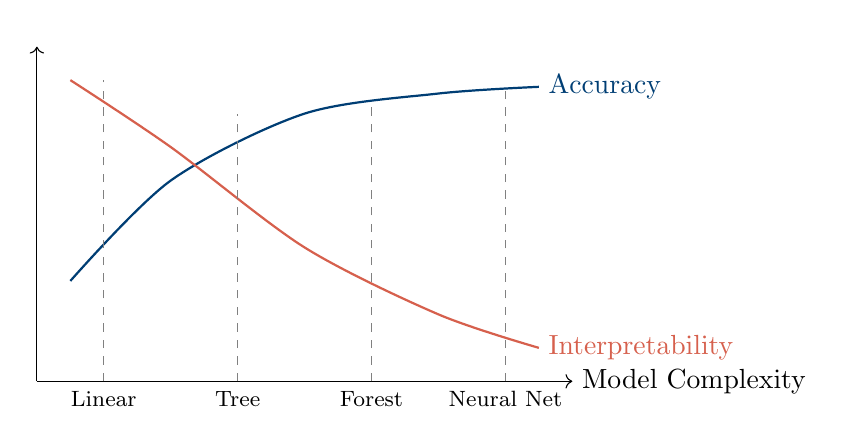
\begin{tikzpicture}[scale=0.85]
    % Axes
    \draw[->] (0,0) -- (8,0) node[right] {Model Complexity};
    \draw[->] (0,0) -- (0,5) node[above] {};

    % Accuracy curve
    \draw[thick, ThemeBlue] plot[smooth] coordinates {(0.5,1.5) (2,3) (4,4) (6,4.3) (7.5,4.4)};
    \node[ThemeBlue, right] at (7.5,4.4) {Accuracy};

    % Interpretability curve
    \draw[thick, AccentOrange] plot[smooth] coordinates {(0.5,4.5) (2,3.5) (4,2) (6,1) (7.5,0.5)};
    \node[AccentOrange, right] at (7.5,0.5) {Interpretability};

    % Model labels
    \node[below, font=\footnotesize] at (1,0) {Linear};
    \node[below, font=\footnotesize] at (3,0) {Tree};
    \node[below, font=\footnotesize] at (5,0) {Forest};
    \node[below, font=\footnotesize] at (7,0) {Neural Net};

    % Dashed lines
    \draw[dashed, gray] (1,0) -- (1,4.5);
    \draw[dashed, gray] (3,0) -- (3,4);
    \draw[dashed, gray] (5,0) -- (5,4.2);
    \draw[dashed, gray] (7,0) -- (7,4.4);
  \end{tikzpicture}
  \end{center}

  \vspace{0.3em}
  \textbf{Traditional view:} Must sacrifice accuracy for interpretability.

  \vspace{0.5em}
  \textbf{Modern view:} Use \highlight{post-hoc interpretability methods} to explain complex models!
\end{frame}

%----------------------------------------------------------------------------------------

\begin{frame}{Two Approaches to Interpretability}

  \textbf{1. Inherently Interpretable Models:}
  \begin{itemize}
    \item Linear regression: Coefficients show direction and magnitude
    \item Logistic regression: Odds ratios
    \item Single decision tree: Visual flowchart
    \item Limited complexity $\Rightarrow$ Limited accuracy
  \end{itemize}

  \vspace{1em}
  \textbf{2. Post-Hoc Interpretation of Complex Models:}
  \begin{itemize}
    \item Keep your Random Forest or XGBoost
    \item Apply interpretation methods \emph{after} training
    \item Get the best of both worlds
  \end{itemize}

  \vspace{0.5em}
  \begin{block}{Today's Focus}
    Post-hoc methods: Explain feature importance
  \end{block}
\end{frame}

%----------------------------------------------------------------------------------------

\begin{frame}{Global vs.\ Local Interpretability}

  \highlight{Two different questions:}

  \vspace{1em}
  \begin{columns}[T]
    \column{0.48\textwidth}
    \textbf{Global Interpretability:}

    \vspace{0.3em}
    ``How does the model work \emph{in general}?''

    \vspace{0.5em}
    \begin{itemize}
      \item Which features matter most \emph{overall}?
      \item What is the average effect of each feature?
      \item How do features interact?
    \end{itemize}

    \vspace{0.5em}
    \textit{Methods:} Feature importance, PDP

    \column{0.48\textwidth}
    \textbf{Local Interpretability:}

    \vspace{0.3em}
    ``Why did the model make \emph{this specific} prediction?''

    \vspace{0.5em}
    \begin{itemize}
      \item Why was \emph{this} loan denied?
      \item What drove \emph{this} stock's forecast?
      \item How can \emph{this} applicant improve?
    \end{itemize}

    \vspace{0.5em}
    \textit{Methods:} SHAP, LIME
  \end{columns}

  \vspace{1em}
  \begin{block}{Both Matter}
    Global: Model validation and debugging. Local: Individual explanations.
  \end{block}
\end{frame}

%----------------------------------------------------------------------------------------
\section{Feature Importance Methods}
%----------------------------------------------------------------------------------------

\begin{frame}{What Is Feature Importance?}

  \textbf{Question:} Which features contribute most to the model's predictions?

  \vspace{1em}
  \textbf{Why we care:}
  \begin{itemize}
    \item Identify key drivers of predictions
    \item Detect potential data leakage (suspicious features)
    \item Simplify models by removing unimportant features
    \item Communicate what the model has learned
  \end{itemize}

  \vspace{1em}
  \textbf{Two main approaches:}
  \begin{enumerate}
    \item \textbf{Model-specific:} Built into tree-based models
    \item \textbf{Model-agnostic:} Permutation importance (works for any model)
  \end{enumerate}
\end{frame}

%----------------------------------------------------------------------------------------

\begin{frame}{Tree-Based Feature Importance}

  \textbf{For Random Forest / XGBoost:} Built-in importance measure

  \vspace{0.5em}
  \textbf{From Week 3:} Regression trees split to reduce variance within nodes
  \begin{itemize}
    \item A good split creates child nodes where outcomes are more similar
    \item The improvement = variance before split $-$ weighted variance after
  \end{itemize}

  \vspace{0.5em}
  \textbf{Feature importance idea:}
  \begin{itemize}
    \item Each split reduces variance by some amount
    \item Features that create \emph{bigger} variance reductions are more important
    \item Sum reductions across all splits using that feature, across all trees
  \end{itemize}

  \vspace{0.3em}
  \[
  \text{Importance}(X_j) = \sum_{\text{splits on } X_j} (\text{Variance reduction from split})
 \]

  \vspace{0.3em}
  \textbf{Advantages:} Fast (computed during training).

  \vspace{0.3em}
  \textbf{Disadvantage:} Biased toward \highlight{high-cardinality} and \highlight{correlated} features!
\end{frame}

%----------------------------------------------------------------------------------------

\begin{frame}{Permutation Feature Importance}

  \textbf{Idea:} How much does performance \emph{drop} when we break the relationship between a feature and the target?

  \vspace{1em}
  \textbf{Algorithm:}
  \begin{enumerate}
    \item Train model, compute baseline performance (e.g., $R^2$, AUC)
    \item For each feature $X_j$:
    \begin{enumerate}
      \item Randomly shuffle values of $X_j$ (breaks relationship with $Y$)
      \item Compute performance with shuffled $X_j$
      \item Importance = Baseline $-$ Shuffled performance
    \end{enumerate}
    \item Repeat multiple times and average
  \end{enumerate}

  \vspace{0.5em}
  \begin{block}{Intuition}
    If shuffling $X_j$ hurts performance a lot, then $X_j$ is important.
  \end{block}
\end{frame}

%----------------------------------------------------------------------------------------

\begin{frame}{Permutation Importance: Visualization}

  \begin{center}
  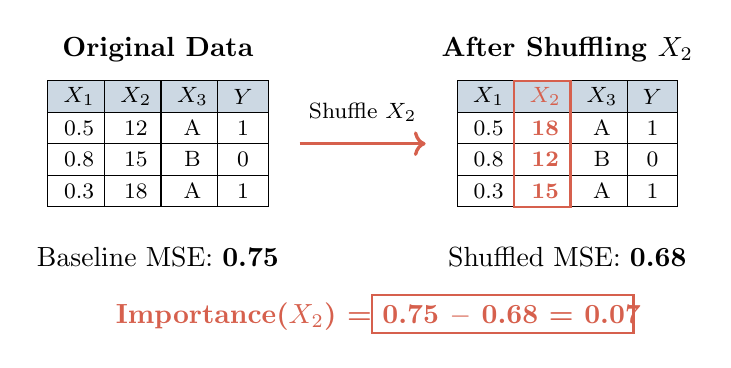
\begin{tikzpicture}[scale=0.8]
    % Original data table
    \node[font=\bfseries] at (1.75, 4.5) {Original Data};

    % Header row
    \fill[ThemeBlue!20] (0,3.5) rectangle (3.5,4);
    \draw (0,3.5) rectangle (3.5,4);
    \node[font=\footnotesize] at (0.5,3.75) {$X_1$};
    \node[font=\footnotesize] at (1.4,3.75) {$X_2$};
    \node[font=\footnotesize] at (2.3,3.75) {$X_3$};
    \node[font=\footnotesize] at (3.1,3.75) {$Y$};

    % Data rows
    \draw (0,3) rectangle (3.5,3.5);
    \node[font=\footnotesize] at (0.5,3.25) {0.5};
    \node[font=\footnotesize] at (1.4,3.25) {12};
    \node[font=\footnotesize] at (2.3,3.25) {A};
    \node[font=\footnotesize] at (3.1,3.25) {1};

    \draw (0,2.5) rectangle (3.5,3);
    \node[font=\footnotesize] at (0.5,2.75) {0.8};
    \node[font=\footnotesize] at (1.4,2.75) {15};
    \node[font=\footnotesize] at (2.3,2.75) {B};
    \node[font=\footnotesize] at (3.1,2.75) {0};

    \draw (0,2) rectangle (3.5,2.5);
    \node[font=\footnotesize] at (0.5,2.25) {0.3};
    \node[font=\footnotesize] at (1.4,2.25) {18};
    \node[font=\footnotesize] at (2.3,2.25) {A};
    \node[font=\footnotesize] at (3.1,2.25) {1};

    % Column lines
    \draw (0.9,2) -- (0.9,4);
    \draw (1.8,2) -- (1.8,4);
    \draw (2.7,2) -- (2.7,4);

    % Arrow
    \draw[->, very thick, AccentOrange] (4, 3) -- (6, 3);
    \node[above, font=\footnotesize] at (5, 3.2) {Shuffle $X_2$};

    % Shuffled data table
    \node[font=\bfseries] at (8.25, 4.5) {After Shuffling $X_2$};

    % Header row
    \fill[ThemeBlue!20] (6.5,3.5) rectangle (10,4);
    \draw (6.5,3.5) rectangle (10,4);
    \node[font=\footnotesize] at (7,3.75) {$X_1$};
    \node[font=\footnotesize, AccentOrange] at (7.9,3.75) {$X_2$};
    \node[font=\footnotesize] at (8.8,3.75) {$X_3$};
    \node[font=\footnotesize] at (9.6,3.75) {$Y$};

    % Data rows - X2 is shuffled
    \draw (6.5,3) rectangle (10,3.5);
    \node[font=\footnotesize] at (7,3.25) {0.5};
    \node[font=\footnotesize, AccentOrange] at (7.9,3.25) {\textbf{18}};
    \node[font=\footnotesize] at (8.8,3.25) {A};
    \node[font=\footnotesize] at (9.6,3.25) {1};

    \draw (6.5,2.5) rectangle (10,3);
    \node[font=\footnotesize] at (7,2.75) {0.8};
    \node[font=\footnotesize, AccentOrange] at (7.9,2.75) {\textbf{12}};
    \node[font=\footnotesize] at (8.8,2.75) {B};
    \node[font=\footnotesize] at (9.6,2.75) {0};

    \draw (6.5,2) rectangle (10,2.5);
    \node[font=\footnotesize] at (7,2.25) {0.3};
    \node[font=\footnotesize, AccentOrange] at (7.9,2.25) {\textbf{15}};
    \node[font=\footnotesize] at (8.8,2.25) {A};
    \node[font=\footnotesize] at (9.6,2.25) {1};

    % Column lines
    \draw (7.4,2) -- (7.4,4);
    \draw (8.3,2) -- (8.3,4);
    \draw (9.2,2) -- (9.2,4);

    % Highlight shuffled column
    \draw[AccentOrange, thick] (7.4,2) rectangle (8.3,4);

    % Performance comparison
    \node at (1.75, 1.2) {Baseline MSE: \textbf{0.75}};
    \node at (8.25, 1.2) {Shuffled MSE: \textbf{0.68}};

    % Result
    \draw[thick, AccentOrange] (5.15, 0) rectangle (9.3, 0.6);
    \node[AccentOrange] at (5.25, 0.25) {\textbf{Importance($X_2$) = 0.75 $-$ 0.68 = 0.07}};
  \end{tikzpicture}
  \end{center}

  \vspace{0.3em}
  Shuffling breaks the relationship between $X_2$ and $Y$. The bigger the performance drop, the more important the feature.
\end{frame}
%----------------------------------------------------------------------------------------

\begin{frame}{Permutation Importance: Advantages and Caveats}

  \textbf{Advantages:}
  \begin{itemize}
    \item \highlight{Model-agnostic:} Works for any model
    \item Computed on \emph{held-out data} (reflects generalization)
    \item No cardinality bias
    \item Intuitive interpretation
  \end{itemize}

  \vspace{1em}
  \textbf{Caveats:}
  \begin{itemize}
    \item \textbf{Correlated features:} Still problematic!
    \begin{itemize}
      \item Shuffling one leaves the other intact
      \item Model can still predict using the correlated feature
      \item Both features appear less important
    \end{itemize}
    \item \textbf{Computational cost:} Need to re-evaluate model many times
    \item \textbf{Extrapolation:} Shuffling can create unrealistic combinations
  \end{itemize}

  \vspace{0.5em}
  \begin{block}{Rule of Thumb}
    Use permutation importance, but be cautious with correlated features.
  \end{block}
\end{frame}

%----------------------------------------------------------------------------------------

\begin{frame}{Feature Importance: Credit Risk Example}

  \textbf{XGBoost model for loan default prediction:}

  \vspace{0.5em}
  \begin{center}
  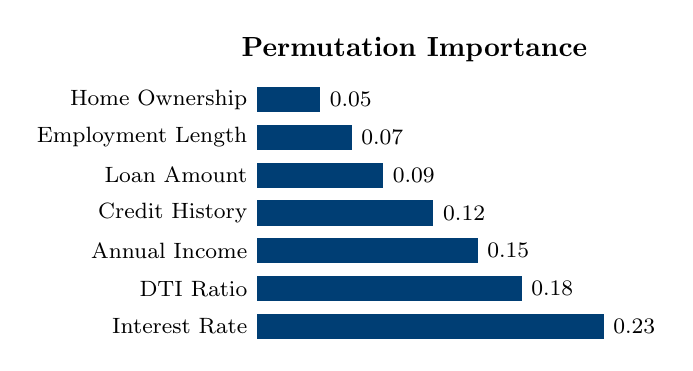
\begin{tikzpicture}[scale=0.8]
    % Bars
    \fill[ThemeBlue] (0,0) rectangle (5.5,0.4);
    \fill[ThemeBlue] (0,0.6) rectangle (4.2,1.0);
    \fill[ThemeBlue] (0,1.2) rectangle (3.5,1.6);
    \fill[ThemeBlue] (0,1.8) rectangle (2.8,2.2);
    \fill[ThemeBlue] (0,2.4) rectangle (2.0,2.8);
    \fill[ThemeBlue] (0,3.0) rectangle (1.5,3.4);
    \fill[ThemeBlue] (0,3.6) rectangle (1.0,4.0);

    % Labels
    \node[left] at (0,0.2) {\footnotesize Interest Rate};
    \node[left] at (0,0.8) {\footnotesize DTI Ratio};
    \node[left] at (0,1.4) {\footnotesize Annual Income};
    \node[left] at (0,2.0) {\footnotesize Credit History};
    \node[left] at (0,2.6) {\footnotesize Loan Amount};
    \node[left] at (0,3.2) {\footnotesize Employment Length};
    \node[left] at (0,3.8) {\footnotesize Home Ownership};

    % Values
    \node[right] at (5.5,0.2) {\footnotesize 0.23};
    \node[right] at (4.2,0.8) {\footnotesize 0.18};
    \node[right] at (3.5,1.4) {\footnotesize 0.15};
    \node[right] at (2.8,2.0) {\footnotesize 0.12};
    \node[right] at (2.0,2.6) {\footnotesize 0.09};
    \node[right] at (1.5,3.2) {\footnotesize 0.07};
    \node[right] at (1.0,3.8) {\footnotesize 0.05};

    % Title
    \node at (2.5, 4.6) {\textbf{Permutation Importance}};
  \end{tikzpicture}
  \end{center}

  \vspace{0.3em}
  \textbf{Interpretation:} Interest rate and debt-to-income (DTI) ratio are the strongest predictors of default. This makes economic sense!
\end{frame}

%----------------------------------------------------------------------------------------
\section{Partial Dependence Plots}
%----------------------------------------------------------------------------------------

\begin{frame}{Beyond Importance: Understanding Relationships}

  \highlight{Feature importance tells us \emph{which} features matter.}

  \vspace{0.5em}
  \textbf{But we also want to know:}
  \begin{itemize}
    \item \emph{How} does the prediction change as a feature changes?
    \item Is the relationship linear? Monotonic? Non-monotonic?
    \item Are there threshold effects or interactions?
  \end{itemize}

  \vspace{1em}
  \textbf{Partial Dependence Plots (PDP):} Show the \highlight{marginal effect} of a feature on predictions.

  \vspace{0.5em}
  \begin{block}{Question PDP Answers}
    ``On average, how does the predicted probability of default change as debt-to-income ratio increases from 10\% to 50\%?''
  \end{block}
\end{frame}

%----------------------------------------------------------------------------------------

\begin{frame}{Partial Dependence: The Idea}

  \textbf{Goal:} Isolate the effect of feature $X_j$ on predictions

  \vspace{1em}
  \textbf{Definition:}
  \[
  \text{PD}(x_j) = \frac{1}{n} \sum_{i=1}^{n} \widehat{f}(x_j, X_{-j}^{(i)})
  \]

  \vspace{0.5em}
  \textbf{In words:}
  \begin{enumerate}
    \item Pick a value $x_j$ for the feature of interest
    \item For \emph{every} observation in the data, set $X_j = x_j$ but keep other features unchanged
    \item Compute predictions for all these modified observations
    \item Average the predictions
  \end{enumerate}

  \vspace{0.5em}
  \textbf{Repeat} for a grid of values of $x_j$ and plot.
\end{frame}

%----------------------------------------------------------------------------------------

\begin{frame}{Partial Dependence: Step-by-Step Example}

    \textbf{Goal:} Isolate the effect of feature $X_j$ on predictions


  \textbf{Suppose we have 3 observations and want PD for DTI ratio:}

  \vspace{0.5em}
  {\small
  \begin{tabular}{cccccl}
    \textbf{Obs} & \textbf{DTI} & \textbf{Income} & \textbf{Rate} & \textbf{...} & \textbf{Original Prediction} \\
    \hline
    1 & 20\% & \$50k & 12\% & ... & $P(\text{def}) = 0.15$ \\
    2 & 35\% & \$80k & 15\% & ... & $P(\text{def}) = 0.25$ \\
    3 & 25\% & \$45k & 10\% & ... & $P(\text{def}) = 0.18$ \\
    \hline
  \end{tabular}
  }

  \vspace{1em}
  \textbf{To compute PD at DTI = 30\%:} Set DTI to 30\% for \emph{all} observations

  \vspace{0.3em}
  {\small
  \begin{tabular}{cccccl}
    \textbf{Obs} & \textbf{DTI} & \textbf{Income} & \textbf{Rate} & \textbf{...} & \textbf{New Prediction} \\
    \hline
    1 & \colorbox{LightBlue}{\textbf{30\%}} & \$50k & 12\% & ... & $P(\text{def}) = 0.22$ \\
    2 & \colorbox{LightBlue}{\textbf{30\%}} & \$80k & 15\% & ... & $P(\text{def}) = 0.20$ \\
    3 & \colorbox{LightBlue}{\textbf{30\%}} & \$45k & 10\% & ... & $P(\text{def}) = 0.24$ \\
    \hline
  \end{tabular}
  }

  \vspace{1em}
  \[
  \text{PD}(\text{DTI}=30\%) = \frac{0.22 + 0.20 + 0.24}{3} = 0.22
  \]

  \textbf{Repeat} for DTI = 10\%, 15\%, 20\%, ..., 50\% to build the full curve.
\end{frame}

%----------------------------------------------------------------------------------------

\begin{frame}{Partial Dependence: Visualization}

  \begin{center}
  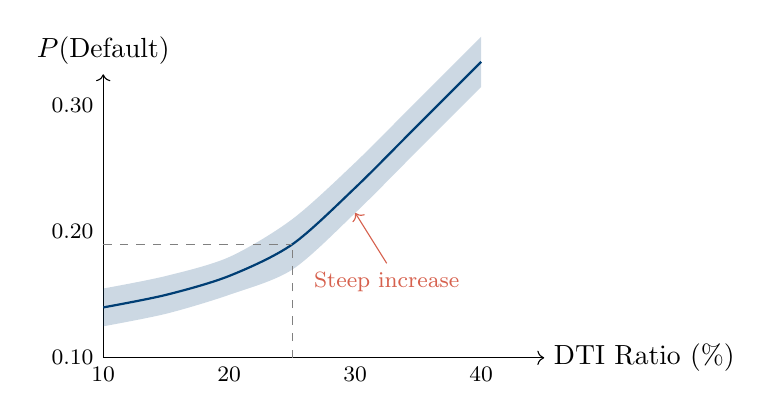
\begin{tikzpicture}[scale=0.8]
    % Axes
    \draw[->] (0,0) -- (7,0) node[right] {DTI Ratio (\%)};
    \draw[->] (0,0) -- (0,4.5) node[above] {$P(\text{Default})$};

    % Axis labels
    \node[below] at (0,0) {\footnotesize 10};
    \node[below] at (2,0) {\footnotesize 20};
    \node[below] at (4,0) {\footnotesize 30};
    \node[below] at (6,0) {\footnotesize 40};

    \node[left] at (0,0) {\footnotesize 0.10};
    \node[left] at (0,2) {\footnotesize 0.20};
    \node[left] at (0,4) {\footnotesize 0.30};

    % PDP curve
    \draw[thick, ThemeBlue] plot[smooth] coordinates {(0,0.8) (1,1.0) (2,1.3) (3,1.8) (4,2.7) (5,3.7) (6,4.7)};

    % Confidence band
    \fill[ThemeBlue, opacity=0.2] plot[smooth] coordinates {(0,0.5) (1,0.7) (2,1.0) (3,1.4) (4,2.3) (5,3.3) (6,4.3)} -- plot[smooth] coordinates {(6,5.1) (5,4.1) (4,3.1) (3,2.2) (2,1.6) (1,1.3) (0,1.1)} -- cycle;

    % Annotation
    \draw[dashed, gray] (3,0) -- (3,1.8);
    \draw[dashed, gray] (0,1.8) -- (3,1.8);
    \node[AccentOrange] at (4.5,1.2) {\footnotesize Steep increase};
    \draw[->, AccentOrange] (4.5,1.5) -- (4,2.3);
  \end{tikzpicture}
  \end{center}

  \vspace{0.3em}
  \textbf{Interpretation:}
  \begin{itemize}
    \item Default probability increases with DTI ratio (as expected)
    \item Relationship is \highlight{non-linear}: steep increase after DTI $>$ 25\%
    \item Shaded area shows variability across the data
  \end{itemize}
\end{frame}

%----------------------------------------------------------------------------------------

\begin{frame}{Two-Way Partial Dependence}

  \textbf{Can also show interactions between two features:}

  \vspace{0.5em}
  \begin{center}
  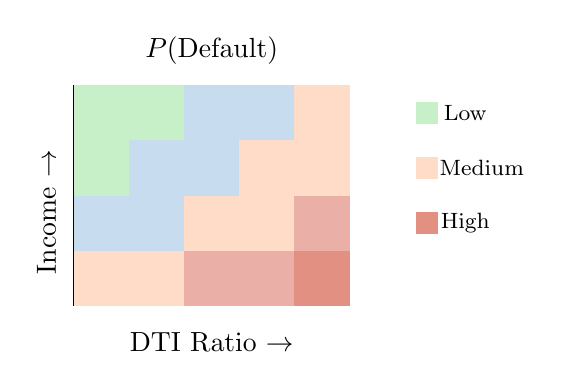
\begin{tikzpicture}[scale=0.7]
    % Heatmap-style visualization
    \draw (0,0) rectangle (5,4);

    % Grid
    \foreach \x in {1,2,3,4} {
      \draw[gray, thin] (\x,0) -- (\x,4);
    }
    \foreach \y in {1,2,3} {
      \draw[gray, thin] (0,\y) -- (5,\y);
    }

    % Color cells (low to high default probability)
    \fill[LightGreen] (0,3) rectangle (1,4);
    \fill[LightGreen] (1,3) rectangle (2,4);
    \fill[LightBlue] (2,3) rectangle (3,4);
    \fill[LightBlue] (3,3) rectangle (4,4);
    \fill[LightOrange] (4,3) rectangle (5,4);

    \fill[LightGreen] (0,2) rectangle (1,3);
    \fill[LightBlue] (1,2) rectangle (2,3);
    \fill[LightBlue] (2,2) rectangle (3,3);
    \fill[LightOrange] (3,2) rectangle (4,3);
    \fill[LightOrange] (4,2) rectangle (5,3);

    \fill[LightBlue] (0,1) rectangle (1,2);
    \fill[LightBlue] (1,1) rectangle (2,2);
    \fill[LightOrange] (2,1) rectangle (3,2);
    \fill[LightOrange] (3,1) rectangle (4,2);
    \fill[AccentOrange!50] (4,1) rectangle (5,2);

    \fill[LightOrange] (0,0) rectangle (1,1);
    \fill[LightOrange] (1,0) rectangle (2,1);
    \fill[AccentOrange!50] (2,0) rectangle (3,1);
    \fill[AccentOrange!50] (3,0) rectangle (4,1);
    \fill[AccentOrange!70] (4,0) rectangle (5,1);

    % Labels
    \node[below] at (2.5,-0.3) {DTI Ratio $\rightarrow$};
    \node[left, rotate=90] at (-0.5,3) {Income $\rightarrow$};

    \node[above] at (2.5,4.2) {$P(\text{Default})$};

    % Legend
    \node at (7.1,3.5) {\footnotesize Low};
    \fill[LightGreen] (6.2,3.3) rectangle (6.6,3.7);
    \node at (7.4,2.5) {\footnotesize Medium};
    \fill[LightOrange] (6.2,2.3) rectangle (6.6,2.7);
    \node at (7.1,1.5) {\footnotesize High};
    \fill[AccentOrange!70] (6.2,1.3) rectangle (6.6,1.7);
  \end{tikzpicture}
  \end{center}

  \vspace{0.3em}
  \textbf{Shows interaction:} High DTI is less problematic for high-income borrowers (can afford the debt service).
\end{frame}

%----------------------------------------------------------------------------------------

\begin{frame}{PDP Limitations: The Independence Assumption}

  \textbf{PDP assumes features are independent.}

  \vspace{0.5em}
  \textbf{Problem:} When computing PD for DTI $= 50\%$, we combine it with \emph{all} observed income levels, including very high incomes.

  \vspace{0.5em}
  But in reality, high DTI and high income rarely occur together!

  \vspace{1em}
  \begin{center}
  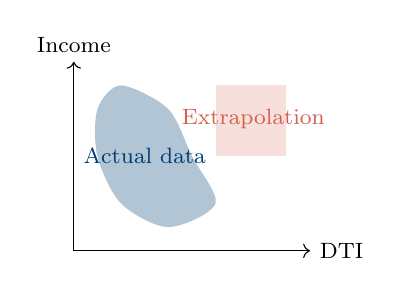
\begin{tikzpicture}[scale=0.6]
    \draw[->] (0,0) -- (5,0) node[right] {\footnotesize DTI};
    \draw[->] (0,0) -- (0,4) node[above] {\footnotesize Income};

    % Actual data region
    \fill[ThemeBlue, opacity=0.3] plot[smooth cycle] coordinates {(0.5,3) (1,3.5) (2,3) (2.5,2) (3,1) (2,0.5) (1,1) (0.5,2)};

    % Extrapolation region
    \fill[AccentOrange, opacity=0.2] (3,2) rectangle (4.5,3.5);

    \node[ThemeBlue] at (1.5,2) {\footnotesize Actual data};
    \node[AccentOrange] at (3.8,2.8) {\footnotesize Extrapolation};
  \end{tikzpicture}
  \end{center}

  \vspace{0.3em}
  \textbf{Result:} PDP may show predictions for \highlight{unrealistic} feature combinations.
\end{frame}

%----------------------------------------------------------------------------------------
\section{SHAP Values}
%----------------------------------------------------------------------------------------

\begin{frame}{The Gold Standard: SHAP}

  \textbf{SHAP = SHapley Additive exPlanations}

  \vspace{1em}
  \textbf{What SHAP provides:}
  \begin{itemize}
    \item \highlight{Local} explanation for each prediction
    \item Additive: contributions sum to prediction
    \item Based on game theory (Shapley values)
    \item Theoretically grounded with desirable properties
  \end{itemize}

  \vspace{1em}
  \textbf{The key question SHAP answers:}

  \vspace{0.3em}
  \begin{quote}
    ``For this specific prediction, how much did each feature contribute to pushing the prediction above or below the average?''
  \end{quote}
\end{frame}

%----------------------------------------------------------------------------------------

\begin{frame}{Shapley Values: Game Theory Foundation}

  \textbf{Origin:} Nobel Prize-winning concept from cooperative game theory (Lloyd Shapley, 1953).

  \vspace{1em}
  \textbf{The game theory analogy:}
  \begin{itemize}
    \item \textbf{Players} = Features
    \item \textbf{Game} = Prediction task
    \item \textbf{Payout} = Prediction minus average prediction
    \item \textbf{Question:} How to fairly divide the ``payout'' among players?
  \end{itemize}

  \vspace{1em}
  \textbf{Shapley's answer:} Give each player their \highlight{average marginal contribution} across all possible coalitions (orderings).
\end{frame}

%----------------------------------------------------------------------------------------

\begin{frame}{Shapley Value: Intuition}

\begin{columns}
\begin{column}{0.5\textwidth}
  \textbf{Example:} ERP forecast
  \begin{itemize}
    \item Average prediction: $0.006$
    \item January 2020 prediction: $-0.041$
    \item Difference to explain: $0.006 - (-0.041) = 0.047$
  \end{itemize}
\end{column}

\begin{column}{0.6\textwidth}
\hspace{5em}SHAP decomposes this as:
\begin{figure}[p]
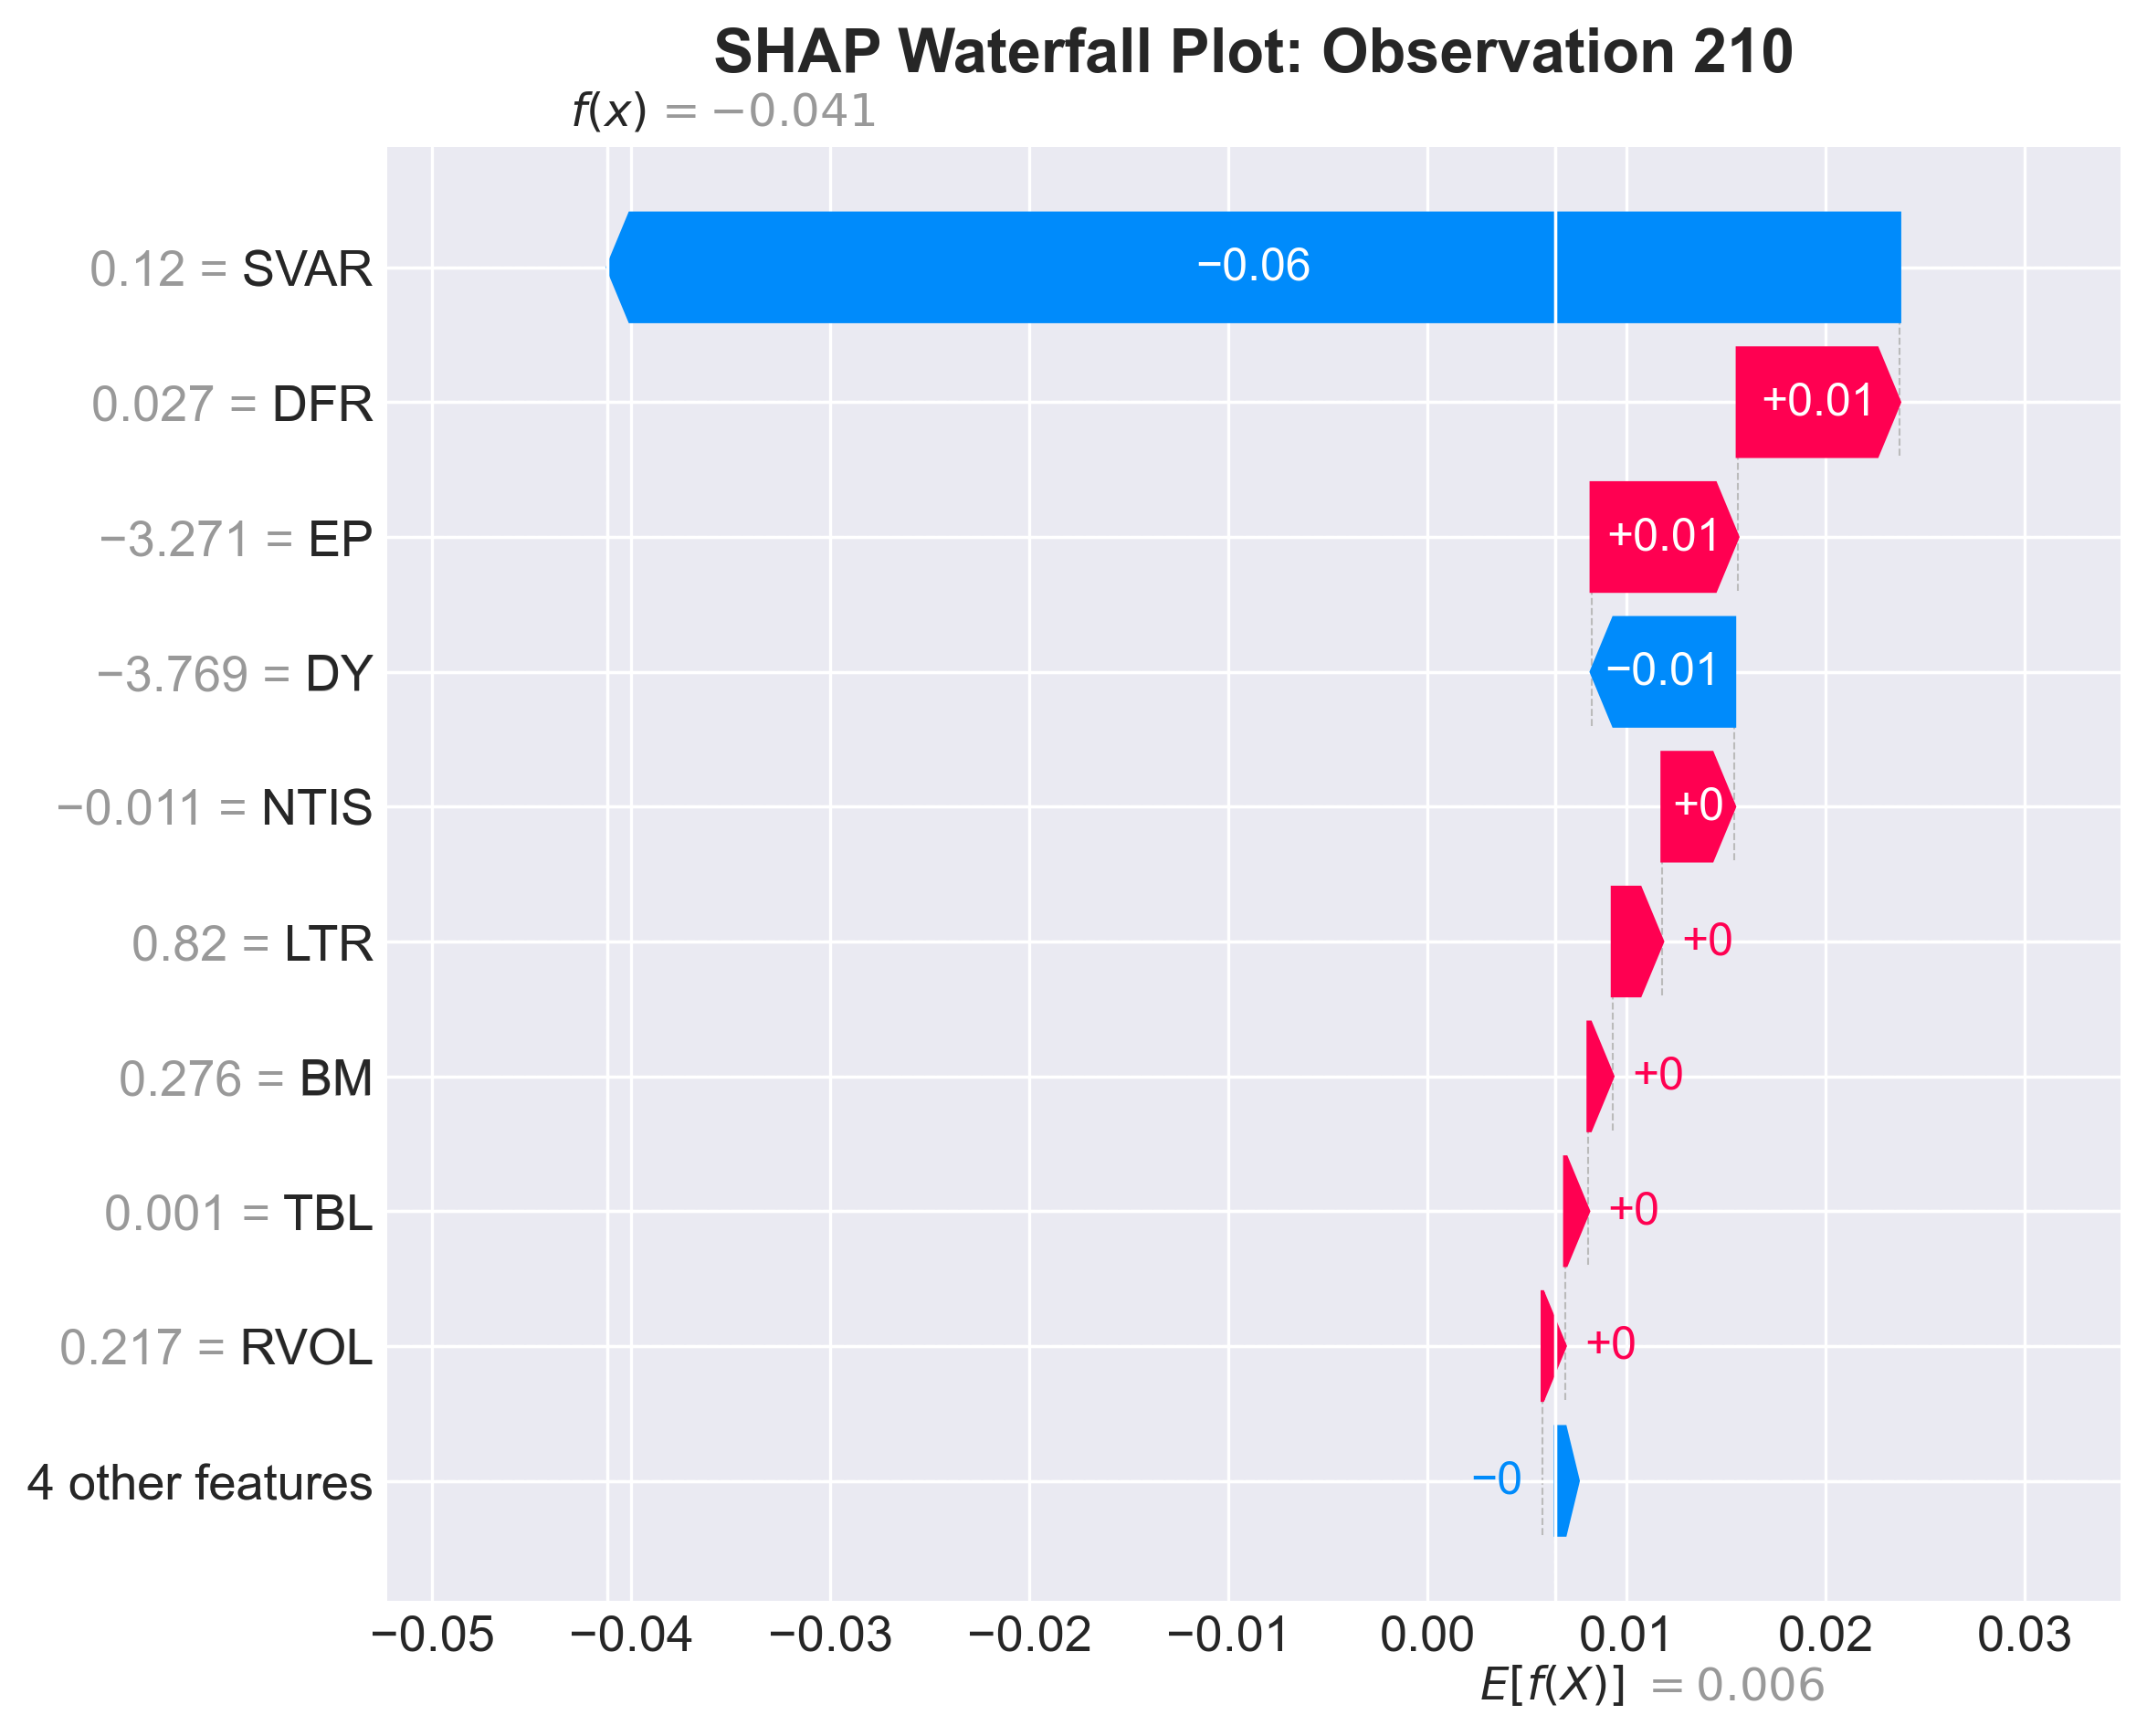
\includegraphics[width=1\textwidth]{Figures/slide23_shap_waterfall.png}
\end{figure}
High SVAR ($-0.06$) push prediction down. High default risk ($+0.01$) and earnings-price ratio ($+0.01$) provide minimal offset.
\end{column}
\end{columns}


\end{frame}

%----------------------------------------------------------------------------------------

\begin{frame}{SHAP: Formal Definition}

  \textbf{For feature $j$ and observation $x$:}
  \[
  \phi_j(x) = \sum_{S \subseteq \{1,\ldots,p\} \setminus \{j\}} \frac{|S|!(p-|S|-1)!}{p!} \left[ f(S \cup \{j\}) - f(S) \right]
  \]

  \vspace{0.5em}
  \textbf{In words:}
  \begin{itemize}
    \item Consider all possible subsets $S$ of features (excluding $j$)
    \item For each subset, compute the marginal contribution of adding $j$
    \item Weight by the number of orderings that produce this subset
    \item Average across all subsets
  \end{itemize}

  \vspace{0.5em}
  \begin{block}{Key Property}
    SHAP values are \highlight{additive}: $f(x) = \phi_0 + \sum_{j=1}^{p} \phi_j(x)$

    where $\phi_0$ is the average prediction.
  \end{block}
\end{frame}

%----------------------------------------------------------------------------------------

\begin{frame}{Why SHAP? Desirable Properties}

  \textbf{SHAP is the \emph{only} method satisfying all of:}

  \vspace{1em}
  \begin{enumerate}
    \item \textbf{Local accuracy:} Contributions sum to prediction
    \[
    f(x) = \phi_0 + \sum_{j=1}^{p} \phi_j(x)
    \]

    \vspace{0.5em}
    \item \textbf{Missingness:} Features not in the model get $\phi_j = 0$

    \vspace{0.5em}
    \item \textbf{Consistency:} If a feature's contribution increases in the model, its SHAP value doesn't decrease

    \vspace{0.5em}
    \item \textbf{Symmetry:} Features that contribute equally get equal SHAP values
  \end{enumerate}

  \vspace{0.5em}
  \begin{block}{Theoretical Foundation}
    These properties uniquely determine the Shapley value formula.
  \end{block}
\end{frame}

%----------------------------------------------------------------------------------------

\begin{frame}{Computing SHAP: The Computational Challenge}

  \textbf{Problem:} Exact Shapley values require summing over $2^p$ subsets!

  \vspace{0.5em}
  With 20 features: $2^{20} \approx 1$ million subsets per prediction.

  \vspace{1em}
  \textbf{Solutions:}

  \vspace{0.5em}
  \begin{center}
  \begin{tabular}{lp{6cm}}
    \toprule
    \textbf{Method} & \textbf{Description} \\
    \midrule
    \textbf{TreeSHAP} & Exact, fast algorithm for tree-based models. $O(TLD^2)$ complexity. \\
    \addlinespace
    \textbf{KernelSHAP} & Model-agnostic approximation using weighted regression. Slower but works for any model. \\
    \addlinespace
    \textbf{DeepSHAP} & Approximation for neural networks using DeepLIFT. \\
    \bottomrule
  \end{tabular}
  \end{center}

  \vspace{0.5em}
  \begin{block}{Practical Advice}
    Use \texttt{TreeSHAP} for tree-based models. Use \texttt{KernelSHAP} for other models.
  \end{block}
\end{frame}

%----------------------------------------------------------------------------------------

\begin{frame}{SHAP Summary Plot: Global View}

\begin{figure}[p]
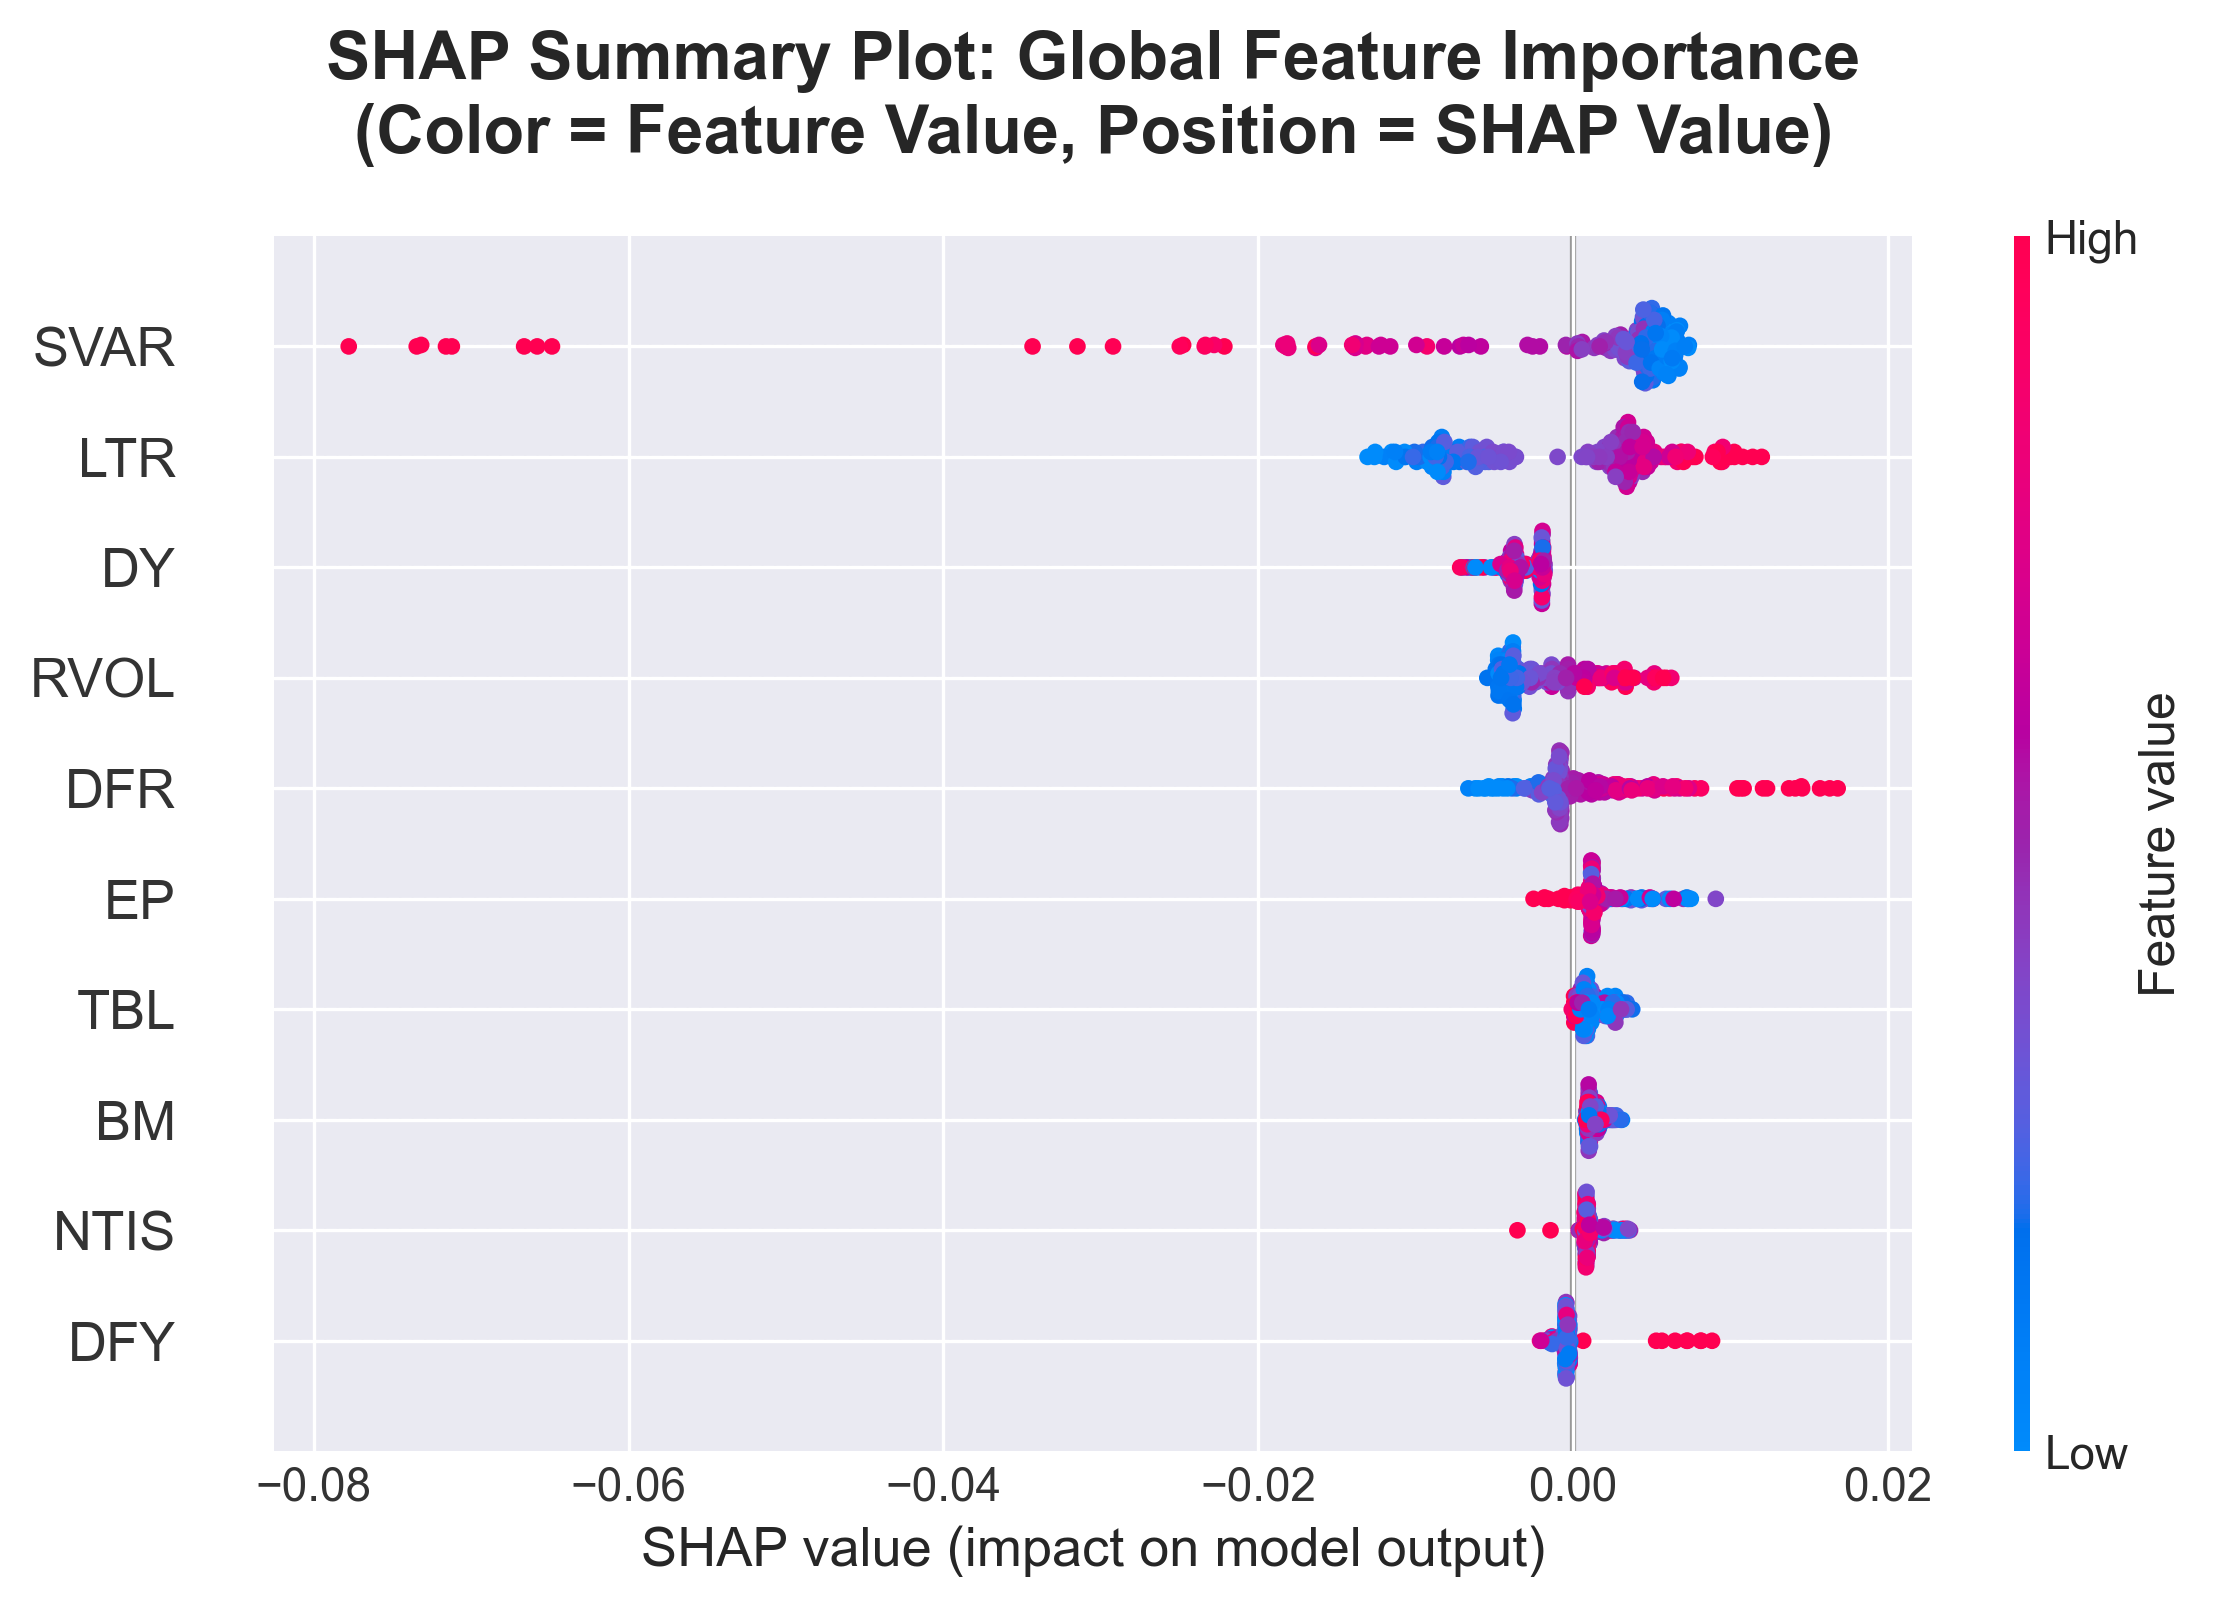
\includegraphics[width=.8\textwidth]{Figures/slide25_shap_summary.png}
\end{figure}

  \vspace{0.3em}
  \textbf{Reading:} High volatility (red dots on left) decreases expected returns. Other predictors have mixed effects.
\end{frame}

%----------------------------------------------------------------------------------------

\begin{frame}{SHAP: Advantages and Limitations}

  \textbf{Advantages:}
  \begin{itemize}
    \item Solid theoretical foundation (game theory)
    \item Local \emph{and} global interpretation
    \item Additive: contributions sum to prediction
    \item Rich visualization options
  \end{itemize}

  \vspace{0.5em}
  \textbf{Limitations:}
  \begin{itemize}
    \item It can be slow for large datasets
    \item Assumes feature independence (like PDP)
    \item Can be sensitive to background data choice
    \item May be complex to explain to non-technical stakeholders
  \end{itemize}

  \vspace{0.5em}
  \begin{block}{Best Practice}
    SHAP is the go-to method for model interpretation in practice. Use TreeSHAP for tree models, supplement with simpler explanations for stakeholders.
  \end{block}
\end{frame}

%----------------------------------------------------------------------------------------
\section{Motivation: Investment Models}
%----------------------------------------------------------------------------------------

\begin{frame}{Why Interpretability Matters for Investment Models}

  \highlight{Interpretability matters above and beyond regulatory requirements}

  \vspace{0.5em}
  \begin{enumerate}
    \item \textbf{Model validation}
    \begin{itemize}
      \item Do feature effects match economic intuition?
      \item Are we capturing signal or noise?
    \end{itemize}

    \vspace{0.3em}
    \item \textbf{Regime detection}
    \begin{itemize}
      \item What's driving the current forecast?
      \item Has the market regime changed?
    \end{itemize}

    \vspace{0.3em}
    \item \textbf{Risk management}
    \begin{itemize}
      \item Why is the model bullish/bearish?
      \item What could make the forecast wrong?
    \end{itemize}

    \vspace{0.3em}
    \item \textbf{Client communication}
    \begin{itemize}
      \item Explaining investment decisions to stakeholders
      \item Building trust in quantitative strategies
    \end{itemize}
  \end{enumerate}
\end{frame}

%----------------------------------------------------------------------------------------

\begin{frame}{The Equity Premium Prediction Problem}

  \textbf{Goal:} Predict next month's excess return on the stock market
  \[
  r_{t+1}^e = r_{t+1}^{mkt} - r_f
  \]

  \vspace{0.5em}
  \textbf{Why might returns be predictable?}
  \begin{itemize}
    \item \textbf{Time-varying risk premia:} Expected returns compensate for risk, and risk varies over the business cycle
    \item \textbf{Behavioral biases:} Investor overreaction, sentiment, slow information diffusion
    \item \textbf{Limits to arbitrage:} Mispricing persists because arbitrage is costly and risky
  \end{itemize}

  \vspace{0.5em}
  \textbf{The academic debate:}
  \begin{itemize}
    \item Goyal \& Welch (2008): Most predictors fail out-of-sample
    \item Campbell \& Thompson (2008): Economically meaningful even with low $R^2$
    \item Gu, Kelly \& Xiu (2020): ML methods improve upon linear models
  \end{itemize}
\end{frame}

%----------------------------------------------------------------------------------------

\begin{frame}{Key Predictor Variables: Details}

  \begin{center}
  \begin{tabular}{llp{5cm}}
    \toprule
    \textbf{Variable} & \textbf{Name} & \textbf{Economic Rationale} \\
    \midrule
    \texttt{d\_p} & Dividend-price ratio & High $\Rightarrow$ cheap market \\
    \texttt{d\_y} & Dividend yield & Income return component \\
    \texttt{e\_p} & Earnings-price ratio & Valuation (inverse P/E) \\
    \texttt{b\_m} & Book-to-market & Value indicator \\
    \texttt{tbl} & T-bill rate & Monetary policy \\
    \texttt{tms} & Term spread & Recession probability \\
    \texttt{dfy} & Default spread & Credit risk premium \\
    \texttt{svar} & Stock variance & Market uncertainty \\
    \texttt{ntis} & Net equity issuance & Corporate timing signal \\
    \texttt{infl} & Inflation & Real return erosion \\
    \bottomrule
  \end{tabular}
  \end{center}

  \vspace{0.3em}
  Plus: \texttt{skvw} (skewness), \texttt{avgcor} (correlation), \texttt{dtoy} (turnover) --- behavioral/technical indicators
\end{frame}

%----------------------------------------------------------------------------------------

\begin{frame}{Target Variable: Market Excess Return}

  \begin{center}
  \begin{tabular}{lr}
    \toprule
    \textbf{Statistic} & \textbf{Value} \\
    \midrule
    Mean & 0.64\% \\
    Std Dev & 4.22\% \\
    Min & $-$22.09\% \\
    Max & 16.19\% \\
    Median & 0.93\% \\
    \bottomrule
  \end{tabular}
  \end{center}

  \vspace{0.5em}
  \textbf{Key observations:}
  \begin{itemize}
    \item Average monthly excess return: 0.64\% ($\approx$ 7.7\% annualized)
    \item High volatility: 4.22\% monthly ($\approx$ 14.6\% annualized)
    \item Left tail: worst month was $-$22\% (October 1987)
    \item \textbf{Signal-to-noise ratio is low!}
  \end{itemize}
\end{frame}

%----------------------------------------------------------------------------------------

\begin{frame}[fragile]{Time-Series Train/Test Split}

  \textbf{Critical:} Use chronological split, not random!

  \vspace{0.3em}
  \fbox{\parbox{0.9\textwidth}{\texttt{\footnotesize
\# Define features and target \\
features = [c for c in df.columns if c not in ['DATE', 'MktRf']] \\
X = df[features].values \\
y = df['MktRf'].values \\
\\
\# Time-series split: first 70\% for training \\
split\_idx = int(len(df) * 0.7)  \# = 577 \\
X\_train, X\_test = X[:split\_idx], X[split\_idx:] \\
y\_train, y\_test = y[:split\_idx], y[split\_idx:] \\
\\
print(f"Training: 1953-04 to 2001-04 (n=577)") \\
print(f"Testing:  2001-05 to 2021-12 (n=248)")
  }}}

  \vspace{0.5em}
  \begin{block}{Why Chronological Split?}
    Random splits cause \highlight{look-ahead bias} --- the model sees ``future'' data during training. This inflates apparent performance.
  \end{block}
\end{frame}

%----------------------------------------------------------------------------------------

\begin{frame}[fragile]{Training the Random Forest}

  \fbox{\parbox{0.9\textwidth}{\texttt{\footnotesize
\# Train Random Forest \\
rf = RandomForestRegressor( \\
\hspace{1cm}n\_estimators=500, \\
\hspace{1cm}max\_depth=5,  \# Shallow trees to avoid overfitting \\
\hspace{1cm}random\_state=42, \\
\hspace{1cm}n\_jobs=-1 \\
) \\
rf.fit(X\_train, y\_train) \\
\\
\# Evaluate \\
from sklearn.metrics import r2\_score \\
y\_pred\_train = rf.predict(X\_train) \\
y\_pred\_test = rf.predict(X\_test) \\
\\
print(f"In-sample R2:  \{r2\_score(y\_train, y\_pred\_train):.4f\}") \\
print(f"Out-of-sample R2: \{r2\_score(y\_test, y\_pred\_test):.4f\}")
  }}}

  \vspace{0.5em}
  \textbf{Results:}
  \begin{itemize}
    \item In-sample $R^2$: \textbf{0.5811} (58\% variance explained)
    \item Out-of-sample $R^2$: \textbf{0.1365} (14\% variance explained)
  \end{itemize}
\end{frame}

%----------------------------------------------------------------------------------------

\begin{frame}{Model Performance Discussion}

  \textbf{In-sample $R^2 = 0.58$ vs.\ Out-of-sample $R^2 = 0.14$}

  \vspace{0.5em}
  \textbf{Is this good?}
  \begin{itemize}
    \item For equity premium prediction: \highlight{Yes!}
    \item Most linear models achieve OOS $R^2 < 0$ (worse than mean)
    \item Campbell \& Thompson (2008): even $R^2 = 0.5\%$ monthly is economically significant
  \end{itemize}

  \vspace{0.5em}
  \textbf{The gap between in-sample and out-of-sample:}
  \begin{itemize}
    \item Some overfitting, but not catastrophic
    \item Shallow trees (max\_depth=5) help regularize
    \item Test period (2001--2021) includes 2008 crisis, COVID --- challenging!
  \end{itemize}

  \vspace{0.5em}
  \begin{block}{Key Question}
    What's driving the predictions? Let's use interpretability methods to find out.
  \end{block}
\end{frame}

%----------------------------------------------------------------------------------------

\begin{frame}{Economic Significance vs.\ Statistical Significance}

  \textbf{Why does $R^2 = 14\%$ matter economically?}

  \vspace{0.5em}
  Consider a mean-variance investor allocating between stocks and bonds:
  \[
 \omega_t = \frac{1}{\gamma} \cdot \frac{\E_t[r_{t+1}^e]}{\sigma^2}
  \]

  \textbf{With predictability:}
  \begin{itemize}
    \item Can time the market: increase weight when expected returns are high
    \item Utility gain from timing $\propto$ $R^2 \times$ Sharpe ratio$^2$
  \end{itemize}

  \vspace{0.5em}
  \textbf{Back-of-envelope calculation:}
  \begin{itemize}
    \item $R^2 = 14\%$ $\Rightarrow$ correlation $\approx 0.37$ between forecast and realized
    \item Annualized Sharpe improvement: $\approx 0.15$--0.25
    \item For a \$1B portfolio: potentially \$15--25M in alpha per year
  \end{itemize}

  \vspace{0.3em}
  \begin{block}{Caveat}
    These gains assume no transaction costs, perfect execution, and stable relationships!
  \end{block}
\end{frame}

%----------------------------------------------------------------------------------------
\section{Opening the Black-Box}
%----------------------------------------------------------------------------------------

\begin{frame}{Feature Importance}

  \begin{center}
  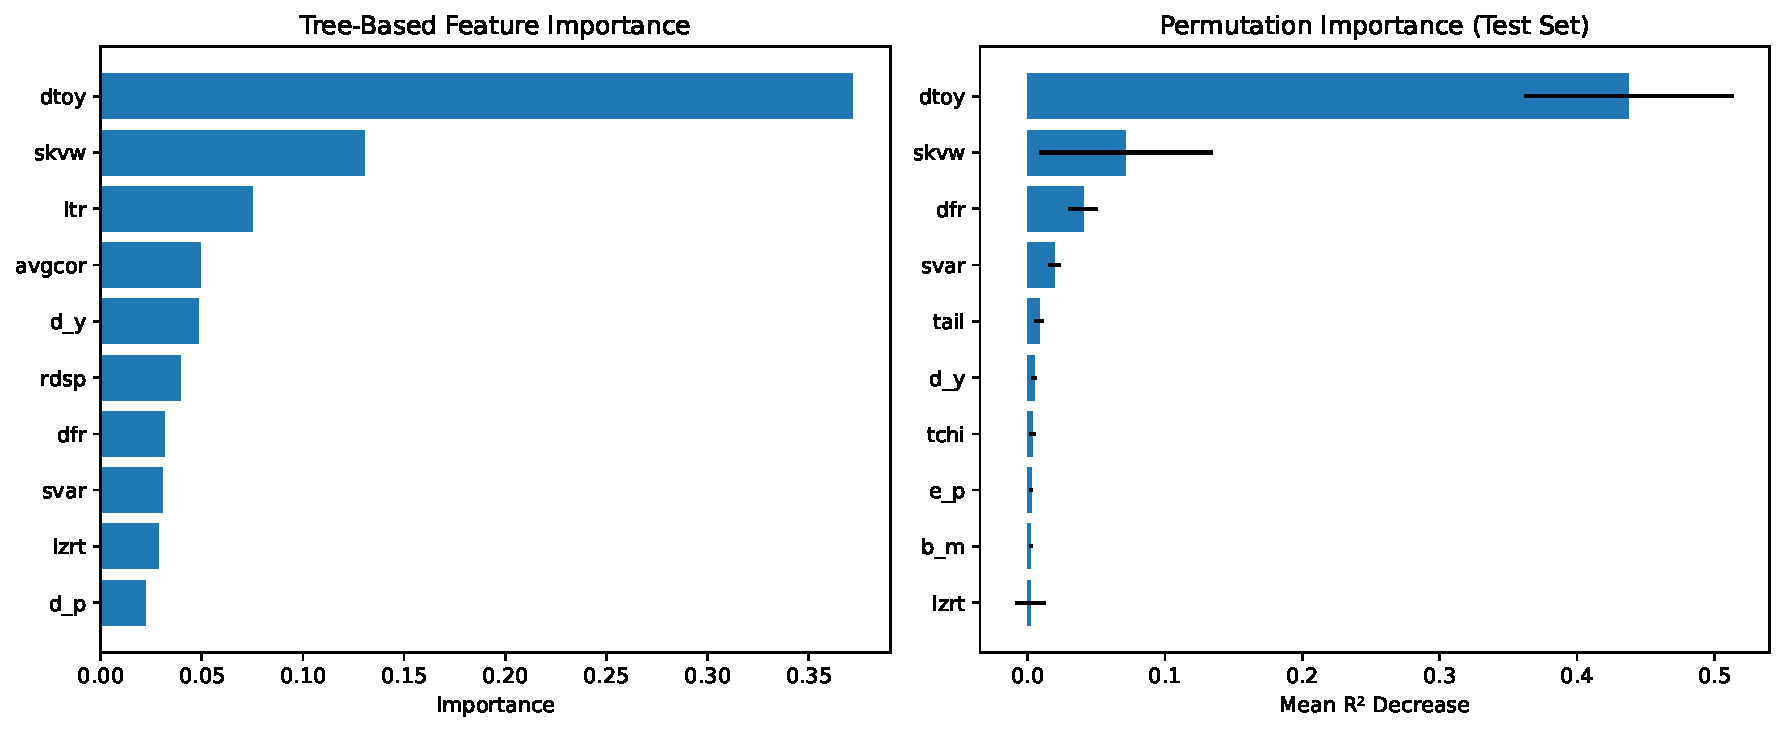
\includegraphics[width=1\textwidth]{Figures/feature_importance_comparison.pdf}
  \end{center}

  \vspace{0.3em}
  \textbf{Left:} Tree-based (in-sample). \textbf{Right:} Permutation (out-of-sample). \texttt{dtoy} dominates in both!
\end{frame}

%----------------------------------------------------------------------------------------

\begin{frame}{Key Observations from Feature Importance}

  \begin{center}
  \begin{tabular}{lcc}
    \toprule
    \textbf{Feature} & \textbf{Tree-Based Rank} & \textbf{Permutation Rank} \\
    \midrule
    dtoy & 1 & 1 \\
    skvw & 2 & 2 \\
    dfr & 7 & 3 \\
    svar & 8 & 4 \\
    ltr & 3 & 10 \\
    avgcor & 4 & 11 \\
    \bottomrule
  \end{tabular}
  \end{center}

  \vspace{0.5em}
  \textbf{Key observations:}
  \begin{itemize}
    \item \texttt{dtoy} and \texttt{skvw} are top 2 in both methods --- \highlight{robust finding}
    \item \texttt{dfr} (default spread) and \texttt{svar} (volatility) rank higher in permutation
    \begin{itemize}
      \item These capture crisis/stress periods (important OOS)
    \end{itemize}
    \item \texttt{ltr} and \texttt{avgcor} may be overfit in-sample
  \end{itemize}

  \vspace{0.3em}
  \textbf{Recommendation:} Trust permutation importance for model validation.
\end{frame}

%----------------------------------------------------------------------------------------

\begin{frame}{Economic Interpretation of Feature Importance}

  \textbf{Surprising result:} Traditional valuation ratios (d\_p, e\_p, b\_m) rank low!

  \vspace{0.5em}
  \textbf{What dominates instead?}

  \begin{enumerate}
    \item \textbf{dtoy (Detrended Turnover):} Behavioral/sentiment indicator
    \begin{itemize}
      \item High turnover = high trading activity = investor enthusiasm
      \item Related to Baker \& Wurgler's sentiment measures
    \end{itemize}

    \vspace{0.3em}
    \item \textbf{skvw (Skewness):} Crash risk / tail risk
    \begin{itemize}
      \item Investors dislike negative skewness (lottery preferences)
      \item High crash risk $\Rightarrow$ investors demand higher returns
    \end{itemize}

    \vspace{0.3em}
    \item \textbf{dfr, svar:} Stress/volatility indicators
    \begin{itemize}
      \item Capture time-varying risk aversion
      \item Counter-cyclical: high in crises, low in booms
    \end{itemize}
  \end{enumerate}

  \vspace{0.3em}
  \begin{block}{Implication}
    The model relies more on \highlight{behavioral/risk} variables than on \highlight{valuation} ratios. This suggests returns are driven by sentiment and risk premia, not just mean reversion.
  \end{block}
\end{frame}

%----------------------------------------------------------------------------------------

\begin{frame}{PDP: dtoy (Detrended Turnover)}

    \texttt{dtoy}: Detrended turnover --- measures trading activity relative to trend. High values indicate unusual trading volume.
  \begin{center}
  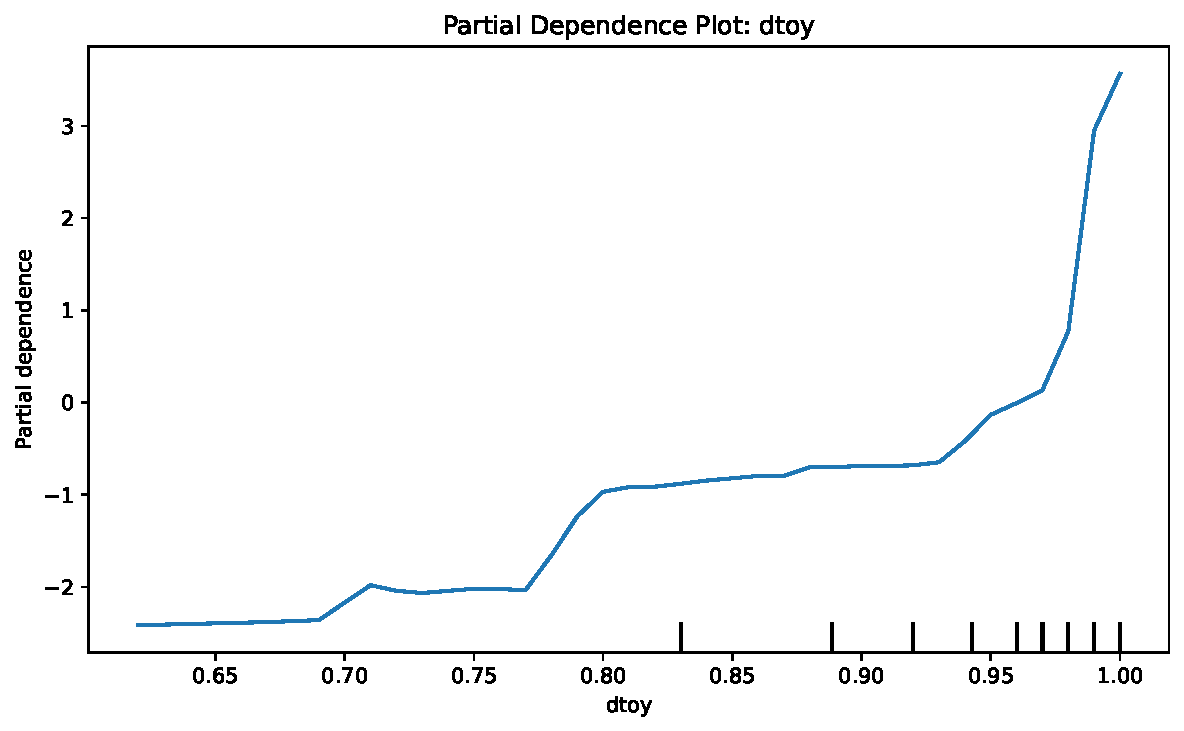
\includegraphics[width=0.75\textwidth]{Figures/pdp_dtoy.pdf}
  \end{center}

  \vspace{0.3em}
  \textbf{Interpretation:} Low turnover $\rightarrow$ bearish. High turnover $\rightarrow$ very bullish. \highlight{Strongly nonlinear} effect above dtoy = 0.97.
\end{frame}

%----------------------------------------------------------------------------------------

\begin{frame}{PDP: skvw (Market Skewness)}

  \begin{center}
  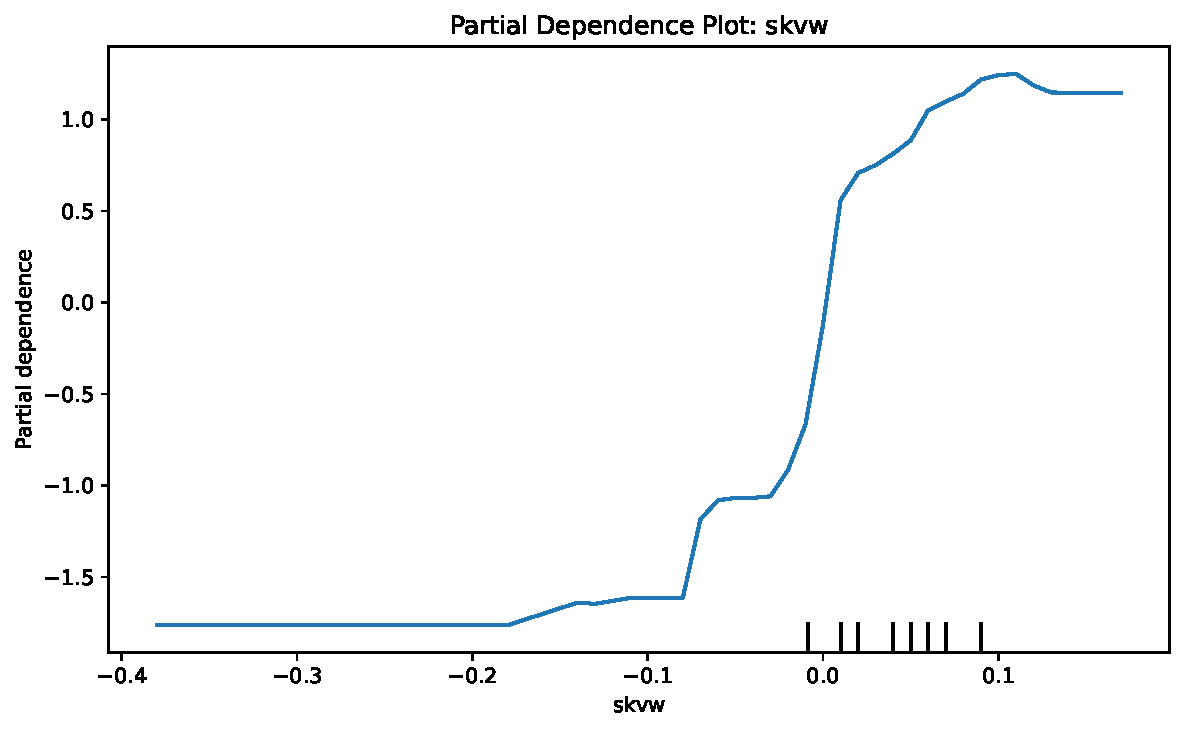
\includegraphics[width=0.75\textwidth]{Figures/pdp_skvw.pdf}
  \end{center}

  \vspace{0.3em}
  \textbf{Interpretation:} Negative skewness (crash risk) $\rightarrow$ bearish. Positive skewness $\rightarrow$ bullish. Effect is monotonic but saturates.
\end{frame}

%----------------------------------------------------------------------------------------

\begin{frame}{Economic Interpretation of PDPs}

  \textbf{dtoy (Detrended Turnover) --- The Sentiment Channel:}
  \begin{itemize}
    \item \textbf{High turnover:} Investors actively trading, optimism, momentum
    \item \textbf{Low turnover:} Apathy, fear, or lack of conviction
    \item Academic link: Baker \& Stein (2004) --- liquidity as sentiment proxy
  \end{itemize}

  \vspace{0.5em}
  \textbf{skvw (Market Skewness) --- The Tail Risk Channel:}
  \begin{itemize}
    \item \textbf{Negative skewness:} Left tail risk (crash potential)
    \item Investors are averse to negative skewness (Barberis \& Huang, 2008)
    \item When crash risk is high, investors demand higher expected returns
  \end{itemize}

  \vspace{0.5em}
  \begin{block}{Key Insight}
    The model captures \highlight{time-varying risk premia}: when investors are scared (low turnover, high crash risk), they require higher compensation $\Rightarrow$ expected returns rise.
  \end{block}
\end{frame}

%----------------------------------------------------------------------------------------
\section{SHAP Analysis}
%----------------------------------------------------------------------------------------

\begin{frame}{SHAP Summary Plot: Bar Chart}

  \begin{center}
  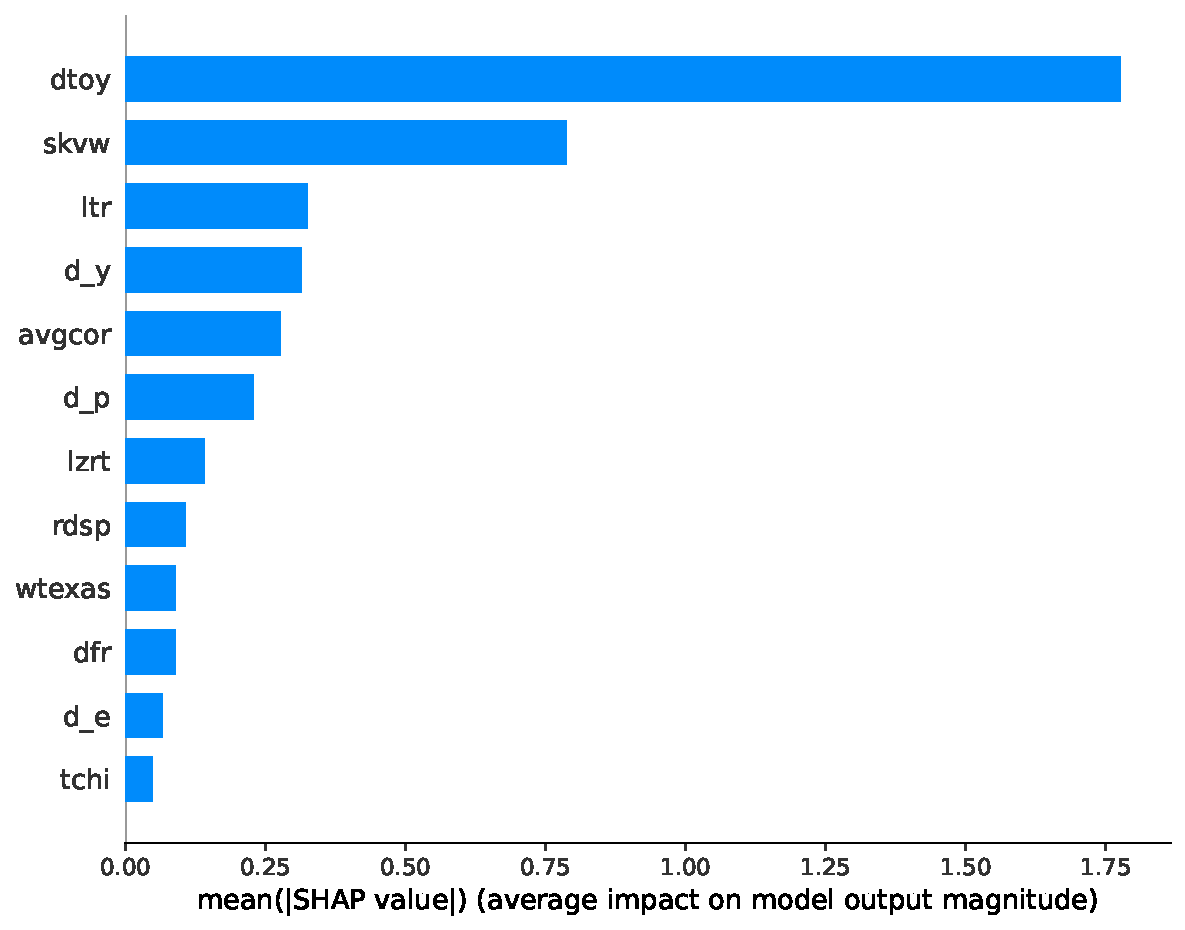
\includegraphics[width=0.75\textwidth]{Figures/shap_summary_bar.pdf}
  \end{center}

  \vspace{0.3em}
  \textbf{Interpretation:} Mean $|\text{SHAP}|$ shows average impact. \texttt{dtoy} contributes $\pm$1.78 percentage points on average --- huge given baseline is only 0.63\%!
\end{frame}

%----------------------------------------------------------------------------------------

\begin{frame}{SHAP Summary Plot: Beeswarm}

  \begin{center}
  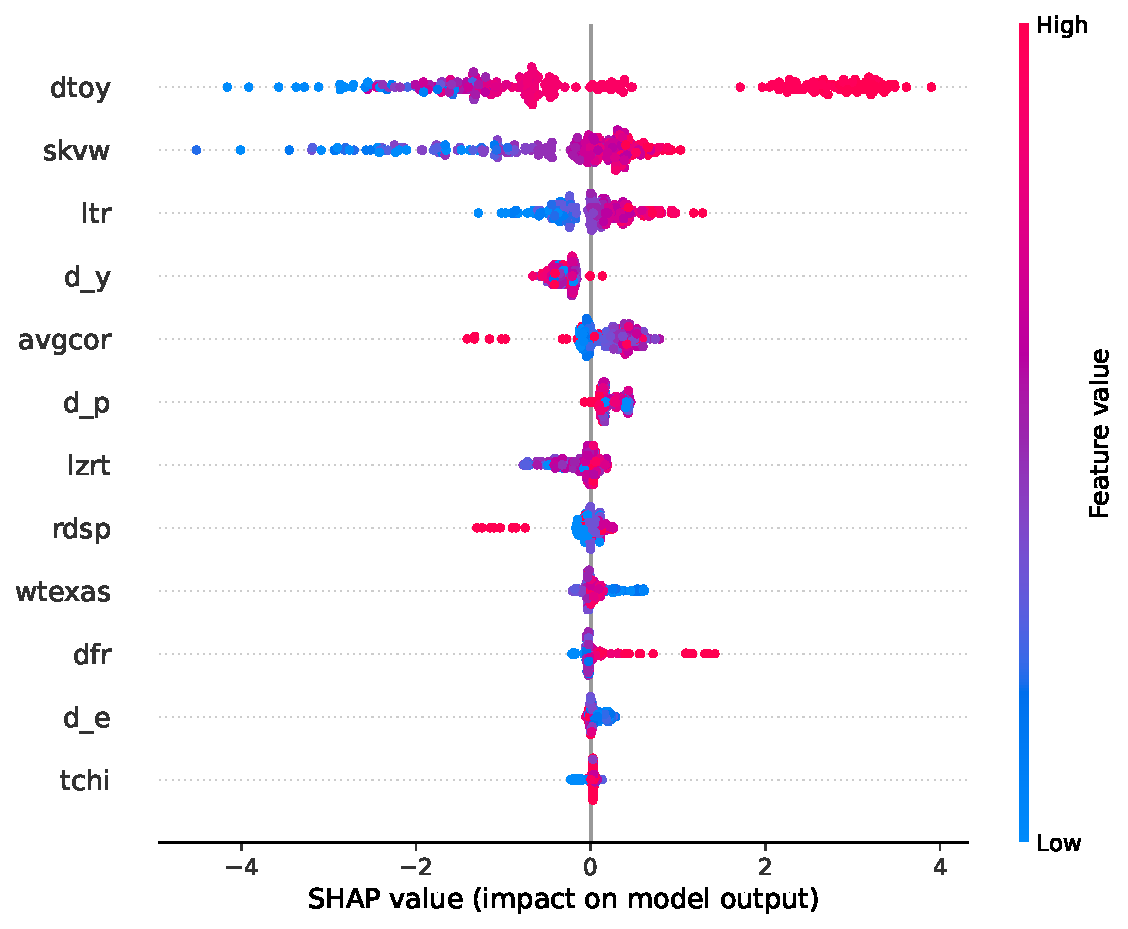
\includegraphics[width=0.75\textwidth]{Figures/shap_summary_dot.pdf}
  \end{center}

  \vspace{0.3em}
  Each dot = one observation. Color = feature value (red=high, blue=low). High \texttt{dtoy} $\rightarrow$ positive SHAP (bullish).
\end{frame}

%----------------------------------------------------------------------------------------

\begin{frame}{SHAP Waterfall: April 2007 (Bullish Signal)}

  \begin{center}
  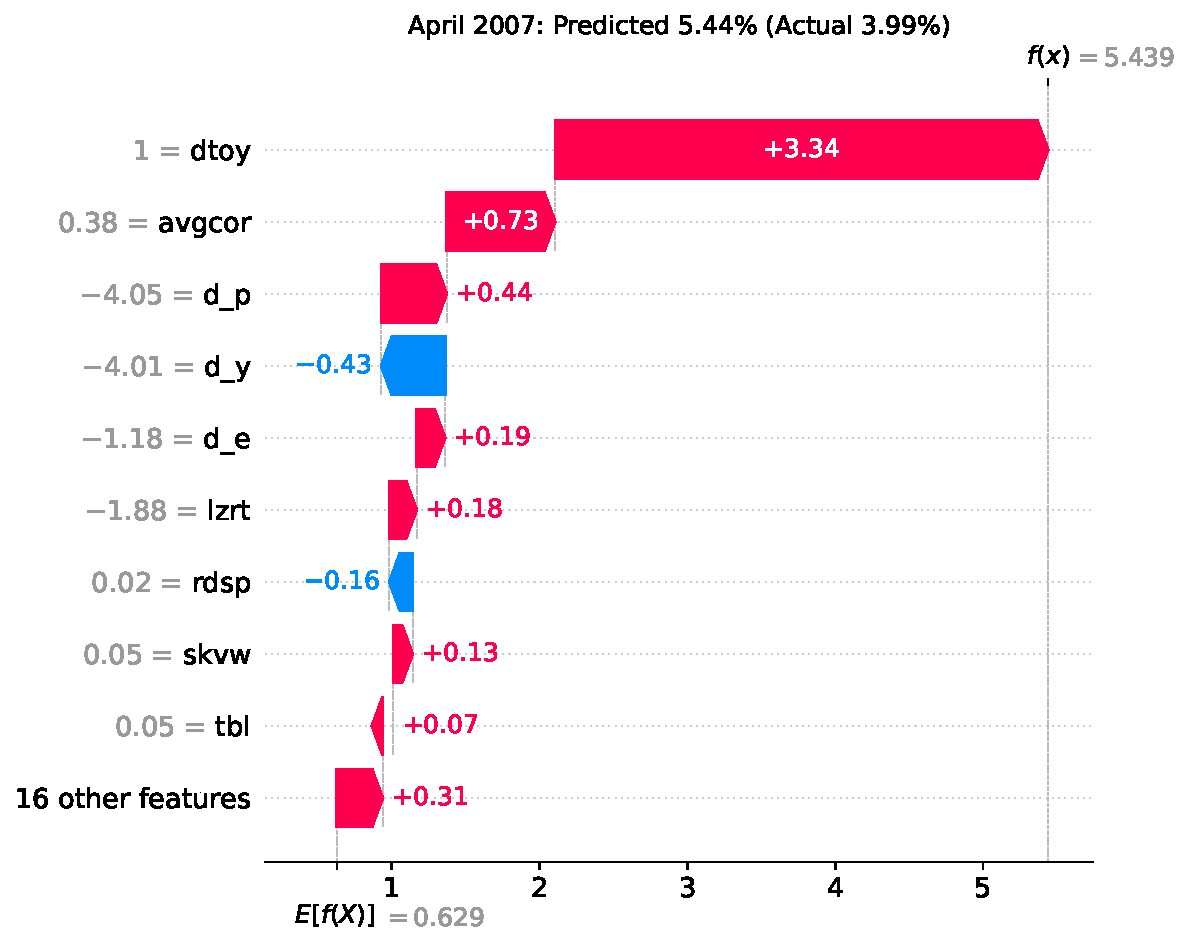
\includegraphics[width=0.75\textwidth]{Figures/shap_waterfall_bullish.pdf}
  \end{center}

  \vspace{0.3em}
  \textbf{Why bullish?} Turnover at maximum (dtoy=1.00) pushed prediction up by +3.34 percentage points!
\end{frame}

%----------------------------------------------------------------------------------------

\begin{frame}{SHAP Waterfall: January 2009 (Bearish Signal)}

  \begin{center}
  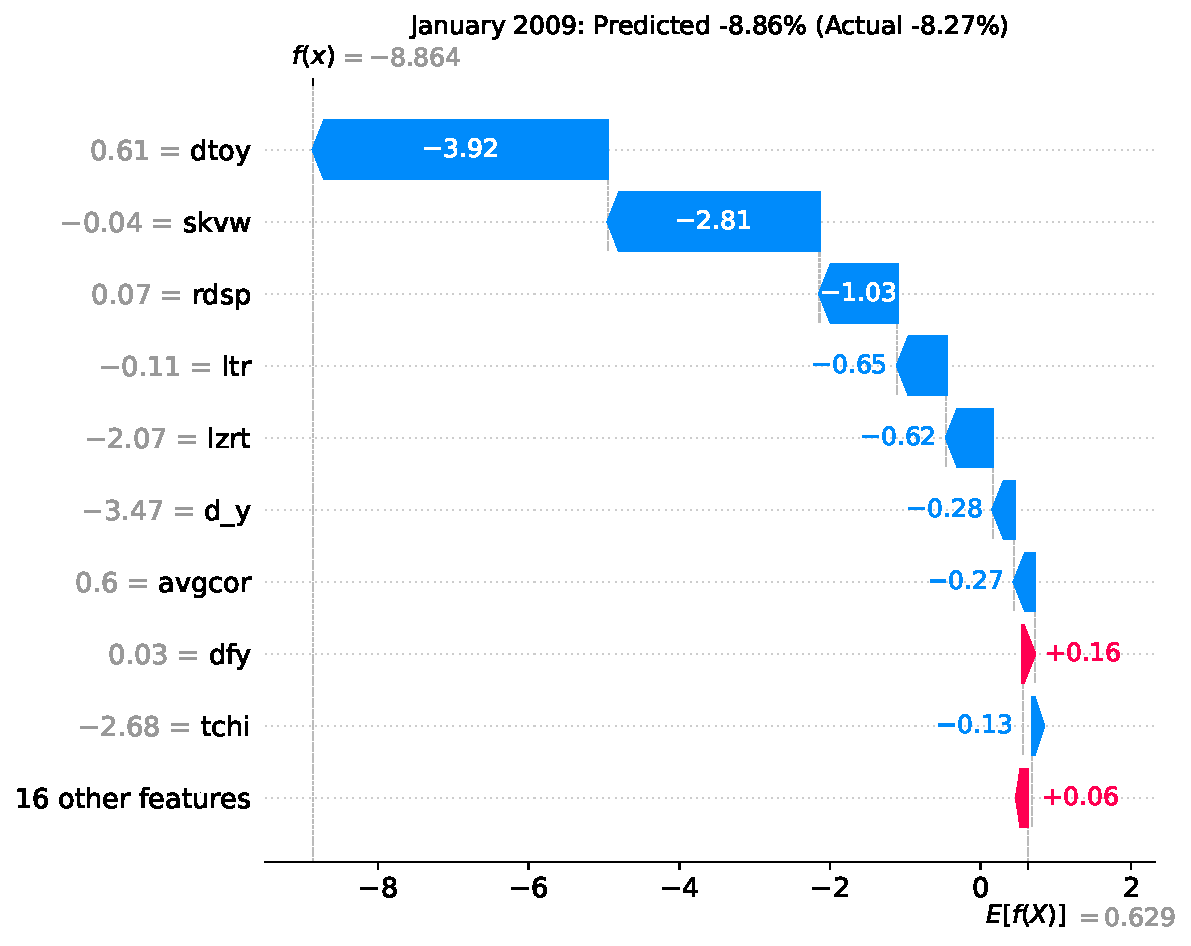
\includegraphics[width=0.75\textwidth]{Figures/shap_waterfall_bearish.pdf}
  \end{center}

  \vspace{0.3em}
  \textbf{Why bearish?} Low turnover, negative skewness, credit stress. Model correctly identified the financial crisis!
\end{frame}

%----------------------------------------------------------------------------------------

\begin{frame}{SHAP Dependence Plot: dtoy}

  \begin{center}
  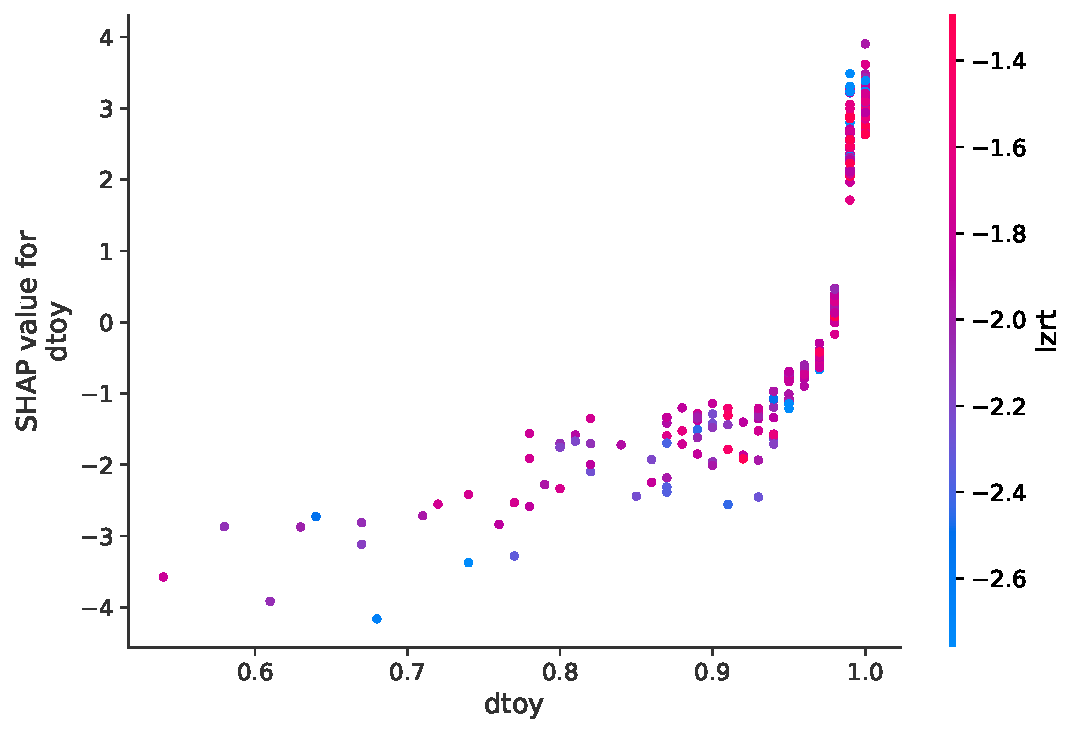
\includegraphics[width=0.75\textwidth]{Figures/shap_dependence_dtoy.pdf}
  \end{center}

  \vspace{0.3em}
  SHAP value vs.\ feature value reveals the nonlinear relationship. Color shows interaction with another feature.
\end{frame}

%----------------------------------------------------------------------------------------

\begin{frame}{Validating the Model: Do Effects Match Theory?}

  \highlight{SHAP reveals the effects direction: do they make economic sense?}

  \vspace{0.3em}
  \begin{center}
  \begin{tabular}{lccp{3.5cm}}
    \toprule
    \textbf{Feature} & \textbf{High $\rightarrow$} & \textbf{Theory} & \textbf{Mechanism} \\
    \midrule
    dtoy & Bullish & Behavioral & Sentiment/momentum \\
    skvw & Bullish & Risk-based & Low crash risk \\
    avgcor & Bullish & Behavioral & Herding/optimism \\
    dfr & Bearish & Risk-based & Credit stress \\
    svar & Bearish & Risk-based & Uncertainty \\
    d\_y & Bullish & Valuation & Mean reversion \\
    \bottomrule
  \end{tabular}
  \end{center}

  \vspace{0.3em}
  \textbf{All effects align with theory!} This increases confidence that:
  \begin{itemize}
    \item The model captures real economic relationships, not spurious patterns
    \item Predictions can be trusted when economic conditions match training data
    \item We can anticipate when the model might fail (regime changes)
  \end{itemize}
\end{frame}

%----------------------------------------------------------------------------------------

\begin{frame}{Case Study: The 2007--2009 Financial Crisis}

  \textbf{Does the model capture known economic events?}

  \vspace{0.5em}
  \textbf{April 2007 (Pre-crisis peak):}
  \begin{itemize}
    \item dtoy = 1.00 (maximum turnover) --- ``irrational exuberance''
    \item avgcor = 0.38 (high) --- herding behavior
    \item Model prediction: +5.44\% (bullish)
    \item \textbf{Economic interpretation:} Sentiment-driven rally, classic late-cycle behavior
  \end{itemize}

  \vspace{0.5em}
  \textbf{January 2009 (Crisis trough):}
  \begin{itemize}
    \item dtoy = 0.61 (low turnover) --- fear, paralysis
    \item skvw = $-$0.04 (negative) --- crash risk elevated
    \item dfr elevated --- credit markets frozen
    \item Model prediction: $-$8.86\% (bearish)
    \item \textbf{Economic interpretation:} Flight to quality, deleveraging, fire sales
  \end{itemize}

  \vspace{0.3em}
  \begin{block}{Insight}
    Interpretability lets us \highlight{tell an economic story} about each prediction!
  \end{block}
\end{frame}

%----------------------------------------------------------------------------------------
\section{Portfolio Implications}
%----------------------------------------------------------------------------------------

\begin{frame}{From Prediction to Portfolio}

  \textbf{How would an investor use this model?}

  \vspace{0.5em}
  \textbf{Simple market timing strategy:}
  \begin{itemize}
    \item If $\hat{r}_{t+1}^e > \bar{r}$: Overweight equities
    \item If $\hat{r}_{t+1}^e < \bar{r}$: Underweight equities (or go to cash)
  \end{itemize}

  \vspace{0.5em}
  \textbf{Interpretability helps with:}
  \begin{enumerate}
    \item \textbf{Position sizing:} Large positions only when drivers are clear
    \item \textbf{Risk management:} Know which factors could reverse the signal
    \item \textbf{Regime awareness:} Recognize when the model is in/out of regime
    \item \textbf{Client communication:} Explain why you're bullish/bearish
  \end{enumerate}

  \vspace{0.5em}
  \begin{block}{Example}
    ``We're overweight equities because market turnover is elevated and crash risk is low. Key risk: if credit spreads widen, our signal would flip bearish.''
  \end{block}
\end{frame}

%----------------------------------------------------------------------------------------

\begin{frame}{When to Trust (and Distrust) the Model}

  \textbf{Trust the model when:}
  \begin{itemize}
    \item SHAP decomposition tells a coherent economic story
    \item Dominant features (dtoy, skvw) are the main drivers
    \item Current regime resembles training data
  \end{itemize}

  \vspace{0.5em}
  \textbf{Be cautious when:}
  \begin{itemize}
    \item Prediction is driven by minor/unstable features
    \item Features are at extreme values (extrapolation)
    \item Market structure has changed (e.g., rise of passive investing)
    \item SHAP contributions nearly cancel out (low conviction)
  \end{itemize}

  \vspace{0.5em}
  \begin{block}{Risk Management Principle}
    Use SHAP to compute ``conviction scores'' --- size positions based on how cleanly the prediction is explained by theoretically-grounded factors.
  \end{block}
\end{frame}

%----------------------------------------------------------------------------------------

\begin{frame}{Limitations and Model Risk}

  \textbf{Every model has limitations --- interpretability helps identify them:}

  \vspace{0.5em}
  \begin{enumerate}
    \item \textbf{Structural breaks:}
    \begin{itemize}
      \item Model trained 1953--2001 may not capture post-GFC dynamics
      \item Rise of algorithmic trading, passive investing, QE
    \end{itemize}

    \vspace{0.3em}
    \item \textbf{Crowding:}
    \begin{itemize}
      \item If everyone uses the same predictors, alpha disappears
      \item GWZ predictors are well-known in academia
    \end{itemize}

    \vspace{0.3em}
    \item \textbf{Nonlinear extrapolation:}
    \begin{itemize}
      \item PDP shows extreme nonlinearity for dtoy $>$ 0.97
      \item What happens at dtoy = 1.05? (Never seen in training)
    \end{itemize}

    \vspace{0.3em}
    \item \textbf{Omitted variables:}
    \begin{itemize}
      \item No Fed policy, no geopolitical risk, no ESG factors
    \end{itemize}
  \end{enumerate}
\end{frame}

%----------------------------------------------------------------------------------------
\section{Practical Workflow}
%----------------------------------------------------------------------------------------

\begin{frame}{Interpretability Workflow for Investment Models}

  \textbf{Step 1: Train model with proper validation}
  \begin{itemize}
    \item Time-series split (no look-ahead bias)
    \item Report in-sample AND out-of-sample metrics
  \end{itemize}

  \vspace{0.3em}
  \textbf{Step 2: Feature importance analysis}
  \begin{itemize}
    \item Compare tree-based and permutation importance
    \item Flag features that rank differently (potential overfit)
  \end{itemize}

  \vspace{0.3em}
  \textbf{Step 3: Understand feature effects (PDP)}
  \begin{itemize}
    \item Are effects monotonic? Nonlinear? Threshold effects?
    \item Do they match economic intuition?
  \end{itemize}

  \vspace{0.3em}
  \textbf{Step 4: Explain individual predictions (SHAP)}
  \begin{itemize}
    \item What's driving today's forecast?
    \item Examine extreme predictions carefully
  \end{itemize}
\end{frame}

%----------------------------------------------------------------------------------------

\begin{frame}{Model Documentation Checklist}

  \textbf{For any deployed investment model, document:}

  \vspace{0.3em}
  \begin{center}
  \begin{tabular}{lc}
    \toprule
    \textbf{Item} & \textbf{Completed} \\
    \midrule
    In-sample and OOS performance metrics & $\square$ \\
    Time-series validation methodology & $\square$ \\
    Feature importance (both methods) & $\square$ \\
    PDP for top 5 features & $\square$ \\
    SHAP summary plot & $\square$ \\
    Example SHAP force plots (bull/bear) & $\square$ \\
    Economic interpretation of effects & $\square$ \\
    Known limitations and failure modes & $\square$ \\
    Monitoring plan & $\square$ \\
    \bottomrule
  \end{tabular}
  \end{center}

  \vspace{0.3em}
  This documentation supports model governance, risk management, and client communication.
\end{frame}

%----------------------------------------------------------------------------------------
\section{Summary}
%----------------------------------------------------------------------------------------

\begin{frame}{Key Takeaways}

  \begin{enumerate}
    \item \textbf{Interpretability validates economic content}
    \begin{itemize}
      \item Feature effects should match finance theory
      \item Our model: sentiment (dtoy) and risk (skvw, dfr) dominate
    \end{itemize}

    \vspace{0.3em}
    \item \textbf{Risk vs.\ Behavioral channels}
    \begin{itemize}
      \item Traditional valuation ratios (d\_p, e\_p) are NOT the top predictors
      \item Behavioral/sentiment variables dominate --- supports limits to arbitrage
    \end{itemize}

    \vspace{0.3em}
    \item \textbf{SHAP enables economic storytelling}
    \begin{itemize}
      \item April 2007: Sentiment-driven late-cycle optimism
      \item January 2009: Fear, crash risk, credit stress
    \end{itemize}

    \vspace{0.3em}
    \item \textbf{Practical value for portfolio management}
    \begin{itemize}
      \item Position sizing based on explanation quality
      \item Risk management: know what could flip the signal
      \item Client communication: tell coherent economic stories
    \end{itemize}
  \end{enumerate}
\end{frame}

%----------------------------------------------------------------------------------------

\begin{frame}{Readings and Next Steps}

  \textbf{Readings for Today's Lecture:}
  \begin{itemize}
    \item Goyal \& Welch (2008), ``Equity Premium Prediction,'' \textit{RFS} \hfill \textit{[Supp.]}
    \item Gu, Kelly \& Xiu (2020), ``Empirical Asset Pricing via ML,'' \textit{RFS} \hfill \textit{[Supp.]}
    \item Baker \& Wurgler (2006), ``Investor Sentiment,'' \textit{JF} \hfill \textit{[Supp.]}
  \end{itemize}

  \vspace{0.5em}
  \textbf{Coming Up Next Week:}
  \begin{itemize}
    \item Introduction to neural networks
    \begin{itemize}
      \item Feedforward neural networks: architecture, activation
      \item Backpropagation and gradient descent
      \item Regularization: dropout, early stopping, batch normalization
    \end{itemize}
    \item Financial applications: return prediction, default risk
  \end{itemize}
\end{frame}

%----------------------------------------------------------------------------------------

\begin{frame}[plain]
  \centering
  \vfill
  {\Large Questions?}
  \vfill
\end{frame}

\end{document}
